\documentclass[preprint,12pt]{elsarticle}
\usepackage[T1]{fontenc}
\usepackage{lmodern}
\usepackage{amsmath,amssymb,amsthm}
\usepackage{graphicx}
\usepackage{booktabs}
\usepackage{multirow}
\usepackage{adjustbox}
\usepackage{microtype}
\usepackage[section]{placeins}
\setlength{\emergencystretch}{2em}
\usepackage{algorithm}
\usepackage{algpseudocode}
\usepackage{xcolor}
\usepackage{pifont}
\usepackage{lineno}
\usepackage[hidelinks]{hyperref}
\usepackage[capitalise,nameinlink]{cleveref}

\renewcommand{\topfraction}{0.9}\renewcommand{\textfraction}{0.07}\renewcommand{\floatpagefraction}{0.75}
\setcounter{topnumber}{3}\setcounter{totalnumber}{4}
\newtheorem{theorem}{Theorem}
\newtheorem{lemma}{Lemma}
\newtheorem{proposition}{Proposition}
\newtheorem{corollary}{Corollary}
\newtheorem{assumption}{Assumption}
\theoremstyle{remark}
\newtheorem{remark}{Remark}
\crefname{assumption}{Assumption}{Assumptions}
\crefname{algorithm}{Algorithm}{Algorithms}
\DeclareMathOperator{\Exp}{Exp}
\newcommand{\supp}[1]{Supplementary Section~S#1}

\journal{Image and Vision Computing}

\begin{document}
\begin{frontmatter}

\title{CARA: Conformally calibrated, drift-aware rotation averaging for global structure-from-motion}

\author[a]{Siva Ramakrishna Jeevakala\corref{cor1}}
\ead{jsrkrishna3@gmail.com}
\cortext[cor1]{Corresponding author. ORCID: 0000-0003-0673-055X}
\author[b]{A. P. Siva Kumar}
\ead{sivakumar.cse@jntua.ac.in}
\affiliation[a]{organization={Department of Computer Science and Engineering (AI \& ML), G. Pulla Reddy Engineering College (Autonomous)},
            addressline={Nandyal Road},
            city={Kurnool},
            postcode={518007},
            state={Andhra Pradesh},
            country={India}}
\affiliation[b]{organization={Department of Computer Science and Engineering, JNTUA College of Engineering, Jawaharlal Nehru Technological University Anantapur},
            city={Ananthapuramu},
            postcode={515002},
            state={Andhra Pradesh},
            country={India}}

\begin{abstract}
Global structure-from-motion pipelines now take relative rotations from learned front ends such as VGGT, whose confidences are overconfident and shift under fog, low light or a new sensor. We present CARA, a rotation-averaging method that returns, besides the rotations, calibrated edge gates, a registration set and per-camera error bounds. CARA scores each edge by its uncertainty-normalized cycle-closure error, sets gates and bounds by conformal risk control over scenes with finite-sample guarantees under exchangeability, and rescales uncertainties and the robust kernel by a drift factor estimated without reference poses. On 1,200 synthetic scenes, CARA improves the area under the rotation-error recall curve up to $5^\circ$ over Geman--McClure averaging and GLOMAP's rotation averaging in all six conditions, and its 90\% bounds cover 91.7--97.0\% of cameras under noise shifts. On ETH3D images with VGGT rotations under rendered fog, low light and rain, we show that camera-level front-end failures cancel in every cycle, which explains why bounds under-cover on hard cameras. In a pre-registered run over all 13 ETH3D scenes, difficulty-conditional bounds raise coverage of the hardest cameras from 81.8\% to 92.8\% (Holm-adjusted $p=0.002$) while flagging 42\% of cameras as unreliable, and a learned edge uncertainty separates outlier edges better (AUROC $0.87$ vs.\ $0.70$).
\end{abstract}


\begin{keyword}
Structure from motion \sep Rotation averaging \sep Conformal risk control \sep Uncertainty calibration \sep Distribution shift \sep Learned front ends
\end{keyword}

\end{frontmatter}

\linenumbers

\section{Introduction}\label{sec:intro}

Global structure-from-motion (SfM) estimates all camera rotations at once from pairwise relative rotations, then all positions, and finally refines everything with bundle adjustment. It is the backbone of GLOMAP~\cite{pan2024glomap}, now shipped inside COLMAP~\cite{schoenberger2016sfm}, and of recent hybrids that feed local reconstructions from networks such as VGGT~\cite{wang2025vggt} and MASt3R~\cite{leroy2024mast3r,duisterhof2025mast3rsfm} into global averaging~\cite{pan2026gluemap}. Rotation averaging is the first and most fragile stage: a wrong rotation propagates into translation averaging and bundle adjustment, and symmetric or repetitive scenes produce relative rotations that are wrong yet look correct~\cite{zach2010disambiguating,heinly2014correcting,cai2023doppelgangers}.

Two developments make this fragility more pressing. First, front ends now report uncertainty, and averaging methods can use it~\cite{zhang2023revisiting,olsson2025certifiably}. These methods assume the reported uncertainty is right. For learned front ends it is not: a 2026 audit of seven feed-forward reconstruction models found that confidences rank errors moderately well (median Spearman correlation $0.46$) but are overconfident by a median factor of $2.4$, with nominal 90\% intervals covering only 17--41\% of errors~\cite{deng2026audit}. Second, the level of the error changes with the data: fog, rain, low light or a new sensor raise the error at a fixed reported confidence. A pipeline that trusts the confidence, or a threshold tuned on clean data, then fails silently.

Robust rotation averaging, typically solved by iteratively reweighted least squares (IRLS), handles outliers well when the noise level matches the kernel it was tuned for~\cite{chatterjee2018robust,hartley2011l1,sidhartha2021weights}. It gives no statement about which cameras can be trusted, and it does not notice when the noise level has changed. Conformal prediction~\cite{vovk2005algorithmic,angelopoulos2023gentle} and conformal risk control (CRC)~\cite{angelopoulos2024crc} give distribution-free guarantees, and they have been applied to object pose~\cite{yang2023object}, visual odometry~\cite{stutts2023conformal}, single camera poses~\cite{pathak2026adaptive}, and failure gating for feed-forward reconstruction~\cite{ahmedt2026geocond}. GeoCond~\cite{ahmedt2026geocond} already gates view-graph edges with calibrated risk thresholds derived from learned per-pair features. To our knowledge, no prior work calibrates a cycle-closure test on the view graph by conformal risk control over scenes, gives coverage guarantees for the cameras of a jointly estimated global reconstruction, or detects from the scene itself that the front end's uncertainty has drifted.

\paragraph*{Contributions} We present CARA (Calibrated, conformally gated, drift-Aware Rotation Averaging), a rotation-averaging method for global SfM that returns rotations together with an edge acceptance set, a registration set, and a per-camera error bound. Our contributions are:
\begin{enumerate}
\item A \emph{cycle nonconformity score} that normalizes loop-closure error by recalibrated front-end uncertainty, and \emph{conformal edge and residual gates} whose thresholds are set by conformal risk control over scenes, each with a finite-sample bound on the expected fraction of inlier edges it rejects (\cref{thm:edge,thm:res}).
\item A \emph{label-free drift factor} $\hat\rho$ estimated from cycle closure on the test scene, with a population bracket under outlier contamination (\cref{prop:bracket}), and a small-noise equivariance result showing that rescaling uncertainties and the robust kernel by $\hat\rho$ restores the calibrated behavior under a pure scale shift (\cref{lem:equiv}).
\item \emph{Per-camera error certificates} for a jointly estimated reconstruction, with a finite-sample bound on the expected fraction of registered cameras whose error exceeds its bound (\cref{thm:cam}), together with \emph{consensus bridging}, which lets cameras abstain instead of being attached through unverified edges.
\item \emph{Extensions for camera-level failures}, which cycle tests cannot detect: calibration on scenes with modeled failures, difficulty-conditional bounds with a group-wise guarantee (\cref{cor:group}), and an edge uncertainty learned from several front-end signals, tested in a pre-registered confirmatory run together with their effect on camera positions after translation averaging.
\item An evaluation that reports failures as well as gains: ten-seed synthetic studies with seed-level significance tests, ablations of the main components (\supp{2}), a structured-doppelganger study where cycle tests fail by construction, real data from the 1DSfM Notre Dame collection~\cite{wilson2014robust} with a strictly disjoint calibration/test split and controlled shifts, and real images from ETH3D~\cite{schops2017eth3d} with the VGGT front end under rendered fog, low light and rain, calibrated and tested on different places.
\end{enumerate}

\paragraph*{Scope} CARA addresses the rotation stage. Translation averaging, bundle adjustment and a full comparison with GLOMAP on large image collections are outside the scope of this paper; \cref{sec:discussion} states what they would require. The code, data splits and all result logs are publicly available (see the data availability statement).

\section{Related Work}\label{sec:related}

\paragraph*{Rotation averaging} Hartley \emph{et al.}~\cite{hartley2013rotation} survey the problem. Lie-algebraic averaging~\cite{govindu2004lie} and spectral or chordal relaxations~\cite{martinec2007robust} give fast solutions; convex and certifiable methods give global optimality guarantees under noise assumptions~\cite{eriksson2018rotation,rosen2019sesync,dellaert2020shonan}. Robust variants use $L_1$ costs~\cite{hartley2011l1,chatterjee2013efficient}, iteratively reweighted least squares with Geman--McClure or similar kernels~\cite{chatterjee2018robust,geman1987statistical}, learned edge weights~\cite{purkait2020neurora,sidhartha2021weights}, or hierarchical initialization~\cite{lee2022hara}. Zhang \emph{et al.}~\cite{zhang2023revisiting} add anisotropic two-view uncertainties to robust averaging, and Olsson \emph{et al.}~\cite{olsson2025certifiably} give certifiably optimal solutions for the anisotropic (non-robust) cost. These methods treat the provided uncertainties as correct; CARA recalibrates them, tests them against cycle closure, and detects when their level has drifted.

\paragraph*{View-graph filtering and ambiguity} Loop constraints have long been used to reject wrong relative motions~\cite{zach2010disambiguating,enqvist2011nonsequential,moulon2013global}. Repetitive and symmetric structures produce consistent wrong matches that need specific handling~\cite{heinly2014correcting}; Doppelgangers~\cite{cai2023doppelgangers} and Doppelgangers++~\cite{xiangli2025doppelgangerspp} learn to classify such image pairs, and view-graph pruning improves global SfM on ambiguous scenes~\cite{xu2026pruning}. These filters use fixed or learned thresholds without a statistical statement about what they discard. CARA's gates can be combined with them; its cycle test inherits their blind spot for mutually consistent wrong edges, which we measure in \cref{sec:dop}.

\paragraph*{Global SfM with learned front ends} GLOMAP~\cite{pan2024glomap} replaces incremental registration with rotation averaging followed by joint global positioning. Feed-forward models such as DUSt3R~\cite{wang2024dust3r}, MASt3R~\cite{leroy2024mast3r}, MASt3R-SfM~\cite{duisterhof2025mast3rsfm} and VGGT~\cite{wang2025vggt} predict geometry with per-pixel confidence, and GLUEMAP~\cite{pan2026gluemap} combines their local reconstructions with global motion averaging. The calibration audit of Deng \emph{et al.}~\cite{deng2026audit} shows that these confidences are overconfident and that a two-parameter power law reduces the miscalibration, which motivates our recalibration step.

\paragraph*{Conformal prediction for geometry} Split conformal prediction~\cite{vovk2005algorithmic,lei2018distribution} and conformal risk control~\cite{angelopoulos2024crc} provide finite-sample guarantees under exchangeability; weighted and adaptive variants address covariate shift and online drift~\cite{tibshirani2019covariate,gibbs2021adaptive,barber2023beyond}. In 3D vision, Yang and Pavone~\cite{yang2023object} propagate conformal keypoint sets to object poses, Stutts \emph{et al.}~\cite{stutts2023conformal} conformalize visual odometry, Pathak and Seifi~\cite{pathak2026adaptive} build geodesic conformal sets for egocentric camera poses and show that marginal coverage hides failures on hard frames, and GeoCond~\cite{ahmedt2026geocond} learns a conditioning-aware reliability score for feed-forward reconstruction, gates image pairs with calibrated risk thresholds, and weights pose-graph edges by its uncertainty before averaging. GeoCond is the closest work and already applies calibrated gating to view-graph edges. CARA differs in its signal and its targets: it uses cycle closure normalized by recalibrated uncertainty rather than learned per-pair features, calibrates scene-level losses for the edges and the cameras of a joint reconstruction by conformal risk control, and estimates drift from the test scene without labels. The two are complementary: GeoCond's features could replace or augment $\hat\sigma$ in our score.

\begin{table*}[!htbp]
\centering
\caption{Positioning of CARA against the closest existing work. \ding{51}: provided; $\circ$: partly provided (see note); --: not provided. A: uses front-end uncertainty; B: recalibrates it; C: cycle (loop) consistency test; D: finite-sample, distribution-free calibrated thresholds; E: guarantee on edge decisions of a view graph; F: per-camera error bound for a \emph{jointly} estimated reconstruction; G: label-free drift detection and correction; H: abstains on cameras without consistent support; I: handles mutually consistent doppelganger edges; J: global-optimality certificate.}
\label{tab:positioning}
\setlength{\tabcolsep}{4pt}
\footnotesize
\begin{adjustbox}{max width=\textwidth}\begin{tabular}{llcccccccccc}
\toprule
Method & Problem & A & B & C & D & E & F & G & H & I & J\\
\midrule
Chatterjee \& Govindu~\cite{chatterjee2018robust} & robust rotation averaging & -- & -- & -- & -- & -- & -- & -- & -- & -- & --\\
Zhang \emph{et al.}~\cite{zhang2023revisiting} & uncertainty-aware averaging & \ding{51} & -- & -- & -- & -- & -- & -- & -- & -- & --\\
Olsson \emph{et al.}~\cite{olsson2025certifiably} & certifiable anisotropic averaging & \ding{51} & -- & -- & -- & -- & -- & -- & -- & -- & \ding{51}\\
Zach \emph{et al.}~\cite{zach2010disambiguating} & loop-constraint filtering & -- & -- & \ding{51} & -- & -- & -- & -- & -- & $\circ^{1}$ & --\\
Doppelgangers++~\cite{xiangli2025doppelgangerspp} & look-alike pair classification & -- & -- & -- & -- & -- & -- & -- & -- & \ding{51} & --\\
Yang \& Pavone~\cite{yang2023object} & conformal object pose & -- & -- & -- & \ding{51} & -- & $\circ^{2}$ & -- & -- & -- & --\\
Pathak \& Seifi~\cite{pathak2026adaptive} & conformal egocentric camera pose & -- & -- & -- & \ding{51} & -- & $\circ^{2}$ & -- & -- & -- & --\\
GeoCond~\cite{ahmedt2026geocond} & reliability for feed-forward 3D & $\circ^{3}$ & $\circ^{4}$ & -- & \ding{51} & $\circ^{5}$ & -- & -- & -- & -- & --\\
\midrule
\textbf{CARA (ours)} & calibrated, drift-aware averaging & \ding{51} & \ding{51} & \ding{51} & \ding{51} & \ding{51} & \ding{51} & \ding{51} & \ding{51} & -- & --\\
\bottomrule
\end{tabular}\end{adjustbox}\\[2pt]
\parbox{\textwidth}{\scriptsize $^{1}$Loop constraints address duplicate structure but without a statistical guarantee. $^{2}$Bounds for one object or one frame at a time, not for the cameras of a joint reconstruction. $^{3}$Uses its own learned geometric-conditioning features rather than the front end's uncertainty. $^{4}$Maps its score to a failure probability by Platt scaling. $^{5}$Risk-controlled gating per image pair; no scene-level guarantee on the edges of a view graph.}
\end{table*}


\paragraph*{Summary of novelty} \Cref{tab:positioning} places CARA against the closest work. No single ingredient is new: cycle tests, robust IRLS, power-law recalibration and conformal risk control all exist. What no listed method provides together is (i) a cycle-closure nonconformity score normalized by recalibrated front-end uncertainty and gated by thresholds with a finite-sample guarantee over scenes, (ii) a drift factor estimated from the test scene without reference poses that rescales both the uncertainties and the robust kernel, and (iii) per-camera error bounds for a jointly estimated reconstruction, combined with abstention for cameras without consistent support. CARA does not provide global-optimality certificates, and it does not handle mutually consistent doppelganger edges (\cref{sec:dop}).

\section{Problem Setting}\label{sec:setting}

A \emph{scene} $Z$ consists of a view graph $\mathcal{G}=(\mathcal{V},\mathcal{E})$ with $n=|\mathcal{V}|$ cameras and $m=|\mathcal{E}|$ edges, an observed relative rotation $\tilde R_{ij}\in SO(3)$ for every edge $(i,j)$, and a native uncertainty $\hat\sigma_{ij}>0$ supplied by the front end (a two-view solver, a learned matcher, or a feed-forward network such as VGGT~\cite{wang2025vggt} or MASt3R~\cite{leroy2024mast3r}). The unknown absolute rotations $R_i$ map world to camera coordinates, and the noise-free model is $R_{ij}=R_jR_i^{\top}$. We write $\angle(R)=\arccos\big((\operatorname{tr}R-1)/2\big)$ for the geodesic angle and $\operatorname{Log}:SO(3)\to\mathbb{R}^3$ for the rotation vector. An edge is an \emph{inlier} when $\angle(\tilde R_{ij}R_{ij}^{\top})\le\tau$ for a fixed $\tau$ (we use $\tau=5^\circ$ on real data; in simulation the generator labels outliers). Rotation averaging returns estimates $\hat R_i$, defined up to a global gauge $R_i\mapsto R_iG$, and the per-camera error $e_i=\angle(\hat R_i G^\star R_i^{\top})$ is measured after the best robust gauge alignment $G^\star$.

We ask for three outputs in addition to $\{\hat R_i\}$: (i) edge gates whose expected loss of inlier edges is controlled at user levels; (ii) a registration set $\mathcal{V}_{\mathrm{reg}}\subseteq\mathcal{V}$ that excludes cameras whose pose is not supported by consistent evidence; and (iii) a bound $B_i$ for every registered camera such that the expected fraction of registered cameras with $e_i>B_i$ is at most $\alpha_{\mathrm{cam}}$. We also want (i) and (iii) to remain close to their targets when the test scene is noisier than the calibration scenes, without labels from the test scene.

\paragraph*{Statistical model} Calibration uses scenes with reference rotations. We assume that calibration scenes and the test scene are exchangeable (for example, drawn i.i.d.\ from a distribution over scenes). This is a statement about \emph{scenes}; edges and cameras inside a scene may be arbitrarily dependent. For shifted test scenes we use the following first-order model.

\begin{assumption}[Scale shift]\label{ass:scale}
A shifted scene is generated as $\tilde R_{ij}=R_jR_i^{\top}\operatorname{Exp}(\rho^\star\eta_{ij})$ on inlier edges, where $\{\eta_{ij}\}$ follows the calibration noise law and $\rho^\star\ge 1$ is an unknown scalar; outlier edges are arbitrary. Native uncertainties $\hat\sigma_{ij}$ are \emph{not} rescaled, i.e.\ the front end is unaware of the shift.
\end{assumption}

Assumption~\ref{ass:scale} models what the 2026 calibration audit of feed-forward reconstruction models reports: confidences keep their ranking but their level is wrong, and the error of the level changes with the data~\cite{deng2026audit}. Fog, rain, low light or a new sensor increase error at a fixed reported confidence.

\section{Method}\label{sec:method}

\begin{figure*}[!htbp]
\centering
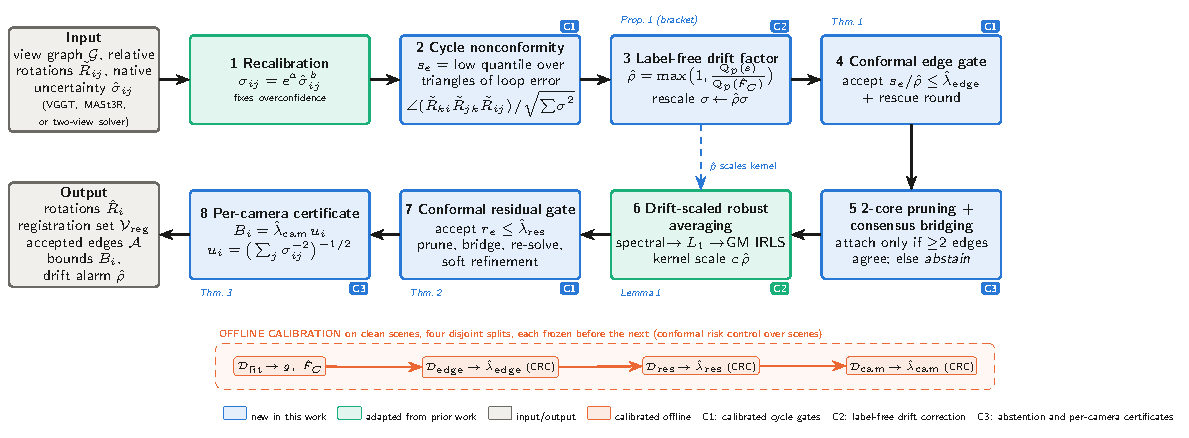
\includegraphics[width=\textwidth]{figs/pipeline.pdf}
\caption{The CARA pipeline. Blue blocks are new in this work and green blocks adapt prior components; tags C1--C3 map blocks to the three contributions and italic labels to the guarantees of \cref{sec:theory}. Offline, four disjoint calibration splits fix the recalibration map $g$ and reference law $\hat F_C$ (used by blocks 1 and 3) and the thresholds $\hat\lambda_{\mathrm{edge}}$, $\hat\lambda_{\mathrm{res}}$ and $\hat\lambda_{\mathrm{cam}}$ (used by blocks 4, 7 and 8). Online, the drift factor $\hat\rho$ from block 3 rescales the uncertainties and the robust kernel of block 6.}
\label{fig:pipeline}
\end{figure*}

\Cref{fig:pipeline} shows the pipeline and \cref{alg:cara} summarizes it. Each step below states its purpose and the design choice that matters for the guarantees.

\subsection{Recalibrated edge uncertainty}
Native uncertainties from learned front ends are rank-informative but overconfident~\cite{deng2026audit}. We fit a two-parameter power law $\sigma_{ij}=g(\hat\sigma_{ij})=e^{a}\hat\sigma_{ij}^{\,b}$ by least squares on $\log\angle(\tilde R_{ij}R_{ij}^\top)$ versus $\log\hat\sigma_{ij}$ over inlier edges of a fitting split $\mathcal{D}_{\mathrm{fit}}$. The constant $e^{a}$ does not affect the calibrated gates and bounds, which are scale-free; it only sets the units of the fixed bridging threshold $\beta$ below. When the front end supplies no uncertainty (as on the 1DSfM data), $\sigma_{ij}$ is constant.

\subsection{Cycle nonconformity score}
For an edge $e=(i,j)$ and a third camera $k$ with edges $(j,k)$ and $(k,i)$, the cycle $C_{ijk}=\tilde R_{ki}\tilde R_{jk}\tilde R_{ij}$ equals the identity for consistent data. We normalize its angle by the predicted cycle spread and aggregate over at most $K$ triangles with a \emph{low} quantile:
\begin{equation}\label{eq:score}
s_e=\operatorname{Q}_{q}\Big\{\frac{\angle(C_{ijk})}{\sqrt{\sigma_{ij}^2+\sigma_{jk}^2+\sigma_{ki}^2}}\;:\;k\in\mathcal{T}_e\Big\},\qquad q=0.25.
\end{equation}
The low quantile protects an inlier edge from triangles contaminated by outliers on the other two edges: with an outlier rate $\varepsilon$, a triangle is clean with probability $(1-\varepsilon)^2$, which is $0.42$ at $\varepsilon=0.35$, so a median would often land on a contaminated triangle. The price is that a group of \emph{mutually consistent} wrong edges passes the test; \cref{sec:dop} measures this failure mode. Edges without any triangle get $s_e=\mathrm{NaN}$ and are deferred to the residual gate.

\subsection{Label-free drift factor}
Let $F_C$ be the law of inlier scores on calibration scenes ($\rho=1$) and $\hat F_C$ its empirical version on $\mathcal{D}_{\mathrm{fit}}$. On a test scene with scores $\{s_e\}$ we estimate
\begin{align}
\hat\rho_{\mathrm{pt}}&=\max\Big(1,\frac{\operatorname{Q}_{p}(\{s_e\})}{\operatorname{Q}_{p}(\hat F_C)}\Big),\quad p=0.2,\label{eq:rho}\\
\hat\rho_{\mathrm{safe}}&=\max\Big(1,\frac{\operatorname{Q}_{p'}(\{s_e\})}{\operatorname{Q}_{(p'-\bar\varepsilon)/(1-\bar\varepsilon)}(\hat F_C)}\Big),\label{eq:rhosafe}
\end{align}
with $p'=0.5$ and $\bar\varepsilon=0.4$, and rescale $\sigma_{ij}\leftarrow\hat\rho\,\sigma_{ij}$, $s_e\leftarrow s_e/\hat\rho$. Cycle closure needs no reference poses, so $\hat\rho$ is computed from the test scene alone. The point estimate uses a low quantile, which is dominated by inliers; the safe estimate is an upper bound on $\rho^\star$ at the population level whenever the outlier fraction is at most $\bar\varepsilon$ (\cref{prop:bracket}). $\hat\rho$ is also a scene-level alarm: $\hat\rho\gg1$ means that the front end's confidence is not valid for this scene.

\subsection{Conformal edge gate}
An edge is accepted in round one if $s_e\le\hat\lambda_{\mathrm{edge}}$ or $s_e=\mathrm{NaN}$. In round two we recompute \eqref{eq:score} using only triangles whose other two edges were accepted, and \emph{rescue} edges whose clean-triangle score falls below $\hat\lambda_{\mathrm{edge}}$. Round two only adds edges, so it cannot increase the loss controlled in \cref{thm:edge}. The threshold $\hat\lambda_{\mathrm{edge}}$ is set by conformal risk control~\cite{angelopoulos2024crc} on a split $\mathcal{D}_{\mathrm{edge}}$ with the per-scene loss
\begin{equation}\label{eq:edgeloss}
L^{\mathrm{edge}}_Z(\lambda)=\frac{1}{|\mathcal{I}_Z|}\sum_{e\in\mathcal{I}_Z}\mathbb{1}[s_e>\lambda],
\end{equation}
where $\mathcal{I}_Z$ is the set of cycle-testable inlier edges of $Z$:
\begin{equation}\label{eq:crc}
\hat\lambda=\inf\Big\{\lambda:\ \tfrac{N}{N+1}\hat R_N(\lambda)+\tfrac{1}{N+1}\le\alpha\Big\},
\end{equation}
with $\hat R_N(\lambda)=\frac1N\sum_{t=1}^{N}L_{Z_t}(\lambda)$ the average loss over the $N$ calibration scenes.

\subsection{Core pruning and consensus bridging}
Gating can leave cameras attached by one or two edges that cannot be checked against anything else. We therefore take the $2$-core of the accepted graph: cameras with fewer than two accepted edges are detached, repeatedly. A detached component $C$ returns to the main component $M$ only through \emph{consensus}: we solve $C$ and $M$ separately, each rejected edge $(a,b)$ with $a\in M$, $b\in C$ implies a gauge $G_{ab}=\hat R_b^{C\top}\tilde R_{ab}\hat R_a^{M}$, and $C$ is attached if at least two such gauges agree, $\angle(G_{ab}^{\top}G_{a'b'})/\sqrt{\sigma_{ab}^2+\sigma_{a'b'}^2}\le\beta$ with a fixed $\beta=3$. Otherwise the cameras of $C$ \emph{abstain} and are reported as unregistered, which is the behavior of incremental SfM when registration fails~\cite{schoenberger2016sfm}. A simpler alternative, ``connect-back'', re-adds the best-scoring rejected edges until the graph is connected; it attaches components through unverified edges and causes catastrophic errors (\supp{2}).

\subsection{Drift-scaled robust averaging}
On the main component we run spectral chordal initialization~\cite{martinec2007robust}, $L_1$-IRLS and Geman--McClure IRLS (GM-IRLS)~\cite{chatterjee2018robust} in the Lie algebra~\cite{govindu2004lie}, with prior weights $w_{ij}\propto\sigma_{ij}^{-2}$ clipped to their 5th--95th percentiles and a kernel scale $c\,\hat\rho$ with $c=5^\circ$. Scaling the kernel with $\hat\rho$ makes the IRLS weights, which depend on $r_{ij}/(c\hat\rho)$, invariant to the noise level under \cref{ass:scale} (\cref{lem:equiv}); the clipped prior weights prevent a single confidently wrong edge from dominating, which is what happens when native confidences enter averaging unmodified (\cref{sec:synth}).

\subsection{Conformal residual gate and final refinement}
After the first solve we compute whitened residuals $r_{ij}=\angle(\hat R_j^{\top}\tilde R_{ij}\hat R_i)/\sigma_{ij}$ for all edges, accept $r_{ij}\le\hat\lambda_{\mathrm{res}}$ (calibrated by \eqref{eq:crc} on a split $\mathcal{D}_{\mathrm{res}}$ with the analogous loss), repeat pruning and bridging, and re-solve. A final Geman--McClure pass over \emph{all} edges among registered cameras, started from the gated solution, recovers inlier redundancy that the hard gates removed. This pass, the pruning and the bridging are outside the guarantees of \cref{sec:theory}.

\subsection{Per-camera certificates}
For a registered camera, $u_i=\big(\sum_{j:(i,j)\in\mathcal{E}_{\mathrm{acc}}}\sigma_{ij}^{-2}\big)^{-1/2}$ is the standard deviation of a Gaussian information proxy. Its scale is wrong for the same reasons as $\hat\sigma$, so we calibrate it: on a split $\mathcal{D}_{\mathrm{cam}}$ we set $\hat\lambda_{\mathrm{cam}}$ by \eqref{eq:crc} with the loss
\begin{equation}\label{eq:camloss}
L^{\mathrm{cam}}_Z(\lambda)=\frac{1}{|\mathcal{V}_{\mathrm{reg}}|}\sum_{i\in\mathcal{V}_{\mathrm{reg}}}\mathbb{1}[e_i>\lambda u_i],
\end{equation}
and report $B_i=\hat\lambda_{\mathrm{cam}}u_i$. Because $u_i$ is built from the $\hat\rho$-scaled $\sigma_{ij}$, the bound widens by $\hat\rho$ on a shifted scene.

\subsection{Extensions for camera-level failures}\label{sec:ext}
A learned front end can misread a whole image: every relative rotation that involves camera $i$ then carries the same error $D_i$, $\tilde R_{ij}=R_{ij}D_i^{\top}$ (or $D_iR_{ij}$ when $i$ is the second index). Such errors cancel in every cycle, $\tilde R_{ki}\tilde R_{jk}\tilde R_{ij}=D_i\,(R_{ki}R_{jk}R_{ij})\,D_i^{\top}$ is conjugate to the true cycle and has the same angle, so no cycle test can detect them and camera $i$ is registered with a wrong pose. A scalar drift factor does not describe them either. We add two optional components that act only on the per-camera bounds; the rotations, gates and registration set are unchanged.

\paragraph*{E1: failure-aware calibration} The calibration scenes are augmented with modeled failures before $\hat\lambda_{\mathrm{cam}}$ is set. Each scene of $\mathcal{D}_{\mathrm{cam}}$ and $\mathcal{D}_{\mathrm{fit}}$ enters five times: unchanged; with inlier edges amounting to 10\% and 20\% of all its edges replaced by uniformly random rotations whose confidences are drawn from the confidences of real outlier edges in $\mathcal{D}_{\mathrm{fit}}$; and with 10\% and 20\% of its cameras misread by a common rotation of $20^\circ$ to $180^\circ$ (plus per-edge noise with $3^\circ$ per axis). The threshold is then the CRC threshold over the augmented $\mathcal{D}_{\mathrm{cam}}$; with E2, $\hat\beta$ and the group boundaries are fitted on the augmented $\mathcal{D}_{\mathrm{fit}}$.

\paragraph*{E2: difficulty-conditional bounds} The normalizer $u_i$ uses only the confidences of the accepted edges. We replace it by
\begin{equation}\label{eq:vnorm}
v_i=u_i\exp\big(\hat\beta^{\top}[1,\,x_i]\big),
\end{equation}
where $x_i$ collects four label-free features of camera $i$ in the final solution: the log median whitened residual of its accepted edges, the fraction of its edges that were rejected, the median log confidence of its edges relative to the scene median, and the log number of accepted edges (the residual is floored at $0.05$ and the exponent in \eqref{eq:vnorm} is clipped to $[-5,5]$). $\hat\beta$ is the least-squares fit of $\log(e_i/u_i)$ on $\mathcal{D}_{\mathrm{fit}}$. The registered cameras are split into $G=3$ groups by $\log v_i$, with group boundaries fixed on $\mathcal{D}_{\mathrm{fit}}$, and each group $g$ receives its own threshold $\hat\lambda_{\mathrm{cam}}^{(g)}$, calibrated by \eqref{eq:crc} over the scenes of $\mathcal{D}_{\mathrm{cam}}$ that have registered cameras in that group, with the loss restricted to those cameras. The bound is $B_i=\hat\lambda^{(g(i))}_{\mathrm{cam}}v_i$. A bound above $30^\circ$ is reported as a \emph{flag}: the method then declares the camera unreliable instead of certifying it. \Cref{sec:v2} evaluates E1 and E2 together with three further extensions: an edge uncertainty learned from several front-end signals (E3), a larger evaluation over all 13 ETH3D scenes (E4), and the effect on camera positions after translation averaging (E5).

\subsection{Calibration protocol}
The four splits $\mathcal{D}_{\mathrm{fit}},\mathcal{D}_{\mathrm{edge}},\mathcal{D}_{\mathrm{res}},\mathcal{D}_{\mathrm{cam}}$ are disjoint. $\mathcal{D}_{\mathrm{fit}}$ fixes $g$ and $\hat F_C$; each later split is processed by the pipeline with all earlier quantities frozen. This ordering is what makes the loss on the test scene exchangeable with the losses on the split that calibrates it. We use $|\mathcal{D}_{\mathrm{fit}}|=20$ and $40$ scenes for each other split; with $N=40$, the term $1/(N+1)$ in \eqref{eq:crc} is $0.024$. Calibration scenes are clean ($\rho^\star=1$).

\begin{algorithm}[t]
\caption{CARA on one test scene}\label{alg:cara}
\begin{algorithmic}[1]
\Require $\mathcal{G}$, $\{\tilde R_{ij},\hat\sigma_{ij}\}$; calibration $(g,\hat F_C,\hat\lambda_{\mathrm{edge}},\hat\lambda_{\mathrm{res}},\hat\lambda_{\mathrm{cam}})$
\State $\sigma_{ij}\gets g(\hat\sigma_{ij})$; compute $s_e$ by \eqref{eq:score}
\State $\hat\rho\gets$ \eqref{eq:rho} or \eqref{eq:rhosafe}; $\sigma\gets\hat\rho\sigma$; $s\gets s/\hat\rho$
\State $\mathcal{A}\gets\{e: s_e\le\hat\lambda_{\mathrm{edge}}\ \text{or}\ s_e=\mathrm{NaN}\}$; rescue with clean-triangle scores
\State $\mathcal{A}\gets$ 2-core$(\mathcal{A})$; consensus bridging $\Rightarrow\mathcal{A},\mathcal{V}_{\mathrm{reg}}$
\State $\hat R\gets$ spectral $\to L_1$-IRLS $\to$ GM-IRLS on $\mathcal{A}$, weights clip$(\sigma^{-2})$, kernel $c\hat\rho$
\State $\mathcal{A}\gets\{e:r_e\le\hat\lambda_{\mathrm{res}}\}$; 2-core; bridging; re-solve
\State GM-IRLS on all edges within $\mathcal{V}_{\mathrm{reg}}$, initialized at $\hat R$
\State $u_i\gets(\sum_{\mathcal{A}\ni(i,j)}\sigma_{ij}^{-2})^{-1/2}$; $B_i\gets\hat\lambda_{\mathrm{cam}}u_i$
\State \Return $\hat R$, $\mathcal{V}_{\mathrm{reg}}$, $\mathcal{A}$, $\{B_i\}$, $\hat\rho$
\end{algorithmic}
\end{algorithm}

\paragraph*{Complexity} Measured runtimes are in \supp{4}. Triangle enumeration costs $O(\sum_{(i,j)}\min(d_i,d_j))$ with $d_i$ the degree, and scoring costs $O(mK)$. Each IRLS iteration solves a sparse $n\times n$ Laplacian system three times (one per axis). Spectral initialization is a dense eigendecomposition for $3n\le1500$ and a Lanczos solve otherwise. Bridging solves each detached component once per attachment.

\section{Guarantees}\label{sec:theory}

Throughout, scenes $Z_1,\dots,Z_N$ of a calibration split and the test scene $Z_{N+1}$ are exchangeable conditionally on the earlier splits, which holds when all scenes are drawn i.i.d.\ and the splits are disjoint. All proofs are in \ref{app:proofs}.

\begin{theorem}[Edge retention]\label{thm:edge}
Let $\hat\lambda_{\mathrm{edge}}$ be given by \eqref{eq:crc} with the loss \eqref{eq:edgeloss} computed on $\mathcal{D}_{\mathrm{edge}}$, with scores produced by lines 1--2 of \cref{alg:cara} (including $\hat\rho$). Then the fraction of cycle-testable inlier edges of the test scene that the edge gate rejects after rescue satisfies
\[
\mathbb{E}\big[L^{\mathrm{edge}}_{Z_{N+1}}\big]\le\alpha_{\mathrm{edge}}.
\]
\end{theorem}

\begin{theorem}[Residual gate and total inlier loss]\label{thm:res}
Let $\hat\lambda_{\mathrm{res}}$ be calibrated on $\mathcal{D}_{\mathrm{res}}$ with the loss $L^{\mathrm{res}}_Z(\lambda)=|\mathcal{I}^{\mathrm{all}}_Z|^{-1}\sum_{e\in\mathcal{I}^{\mathrm{all}}_Z}\mathbb{1}[r_e>\lambda]$, where $r_e=\infty$ if an endpoint is unregistered. Then $\mathbb{E}[L^{\mathrm{res}}_{Z_{N+1}}]\le\alpha_{\mathrm{res}}$.
\end{theorem}

The residual gate re-decides every edge, so \cref{thm:edge,thm:res} control two separate decisions; they are not a bound on a combined set. The 2-core pruning that follows each gate, the consensus bridging and the final refinement over all registered edges are outside both theorems: the accepted set $\mathcal{A}$ that \cref{alg:cara} returns is the residual-gate set after pruning and bridging, and the rotations depend on all edges among registered cameras. We evaluate inlier retention and accuracy of the full pipeline empirically.

\begin{theorem}[Per-camera coverage]\label{thm:cam}
With $\hat\lambda_{\mathrm{cam}}$ calibrated on $\mathcal{D}_{\mathrm{cam}}$ with the loss \eqref{eq:camloss}, the bounds $B_i=\hat\lambda_{\mathrm{cam}}u_i$ satisfy
\[
\mathbb{E}\Big[\frac{1}{|\mathcal{V}_{\mathrm{reg}}|}\sum_{i\in\mathcal{V}_{\mathrm{reg}}}\mathbb{1}[e_i>B_i]\Big]\le\alpha_{\mathrm{cam}},
\]
where the expectation is over calibration and test scenes and $\mathcal{V}_{\mathrm{reg}}$ is the registration set of the test scene.
\end{theorem}

\begin{corollary}[Group-conditional coverage]\label{cor:group}
Let $\hat\beta$ and the group boundaries be fixed on $\mathcal{D}_{\mathrm{fit}}$, and let $\hat\lambda^{(g)}_{\mathrm{cam}}$ be the CRC threshold for the loss $L^{(g)}_Z(\lambda)=\frac{1}{|\mathcal{V}^{(g)}_{\mathrm{reg}}|}\sum_{i\in\mathcal{V}^{(g)}_{\mathrm{reg}}}\mathbb{1}[e_i>\lambda v_i]$ over the scenes of $\mathcal{D}_{\mathrm{cam}}$ in which group $g$ is non-empty. Then, for every group $g$, $\mathbb{E}\big[L^{(g)}_{Z_{\mathrm{test}}}(\hat\lambda^{(g)}_{\mathrm{cam}})\,\big|\,\mathcal{V}^{(g)}_{\mathrm{reg}}(Z_{\mathrm{test}})\neq\emptyset\big]\le\alpha_{\mathrm{cam}}$.
\end{corollary}
\begin{proof}
Given $\mathcal{D}_{\mathrm{fit}}$, the map $Z\mapsto L^{(g)}_Z(\cdot)$ is a fixed function of the scene: non-increasing in $\lambda$ and bounded by $1$. The calibration and test scenes remain exchangeable conditionally on $\mathcal{D}_{\mathrm{fit}}$, and they remain exchangeable after conditioning on the event, a function of each scene alone, that group $g$ is non-empty. The CRC theorem~\cite{angelopoulos2024crc} therefore applies to each group separately over the scenes where it is non-empty, and taking the expectation over $\mathcal{D}_{\mathrm{fit}}$ gives the claim.
\end{proof}
The corollary controls misses within each difficulty group, so the hardest cameras cannot be traded against the easy ones as they can under \cref{thm:cam}; it is still marginal over scenes and conditional on nothing else. The augmentation of E1 changes the calibration distribution, and each calibration scene enters in five correlated copies, so no exact finite-sample statement follows; E1 is a robustness heuristic motivated by the mixture of failure modes, and we evaluate it empirically.

The guarantees are finite-sample and distribution-free under exchangeability of calibration and test scenes, and they do not require the uncertainty proxies $\sigma$ or $u$ to be correct: a poor proxy costs width, not validity. They are \emph{marginal over scenes}: they control the expected fraction of misses in a scene, not the miss probability of a particular camera. They also say nothing about the \emph{accuracy} of $\hat R$, which we evaluate empirically. Coverage refers to registered cameras; abstention is reported separately as the registration rate.

\paragraph*{Shift} Under \cref{ass:scale} the test scene is no longer exchangeable with the calibration scenes, and the theorems do not apply as stated. The next two results explain why rescaling by $\hat\rho$ restores them approximately.

\begin{lemma}[Scale equivariance in the small-noise limit]\label{lem:equiv}
Suppose the shifted scene differs from an unshifted one only as in \cref{ass:scale}: same graph, same outlier edges with the same values, same $\hat\sigma$, inlier noise multiplied by $\rho^\star$. Suppose further that $\hat\rho$ on the shifted scene equals $\rho^\star$ times $\hat\rho$ on the unshifted scene, which requires that the clip $\max(1,\cdot)$ is inactive and that the quantile in \eqref{eq:rho} is attained by an inlier score. Then, to first order in the inlier noise, (a) every inlier cycle rotation vector, and hence every inlier score, scales by $\rho^\star$; (b) the normalized scores $s_e/\hat\rho$ and whitened residuals $r_e$ of inlier edges are unchanged; (c) the $L_1$ and Geman--McClure IRLS weights of inlier edges, which depend on $r/(c\hat\rho)$ or scale uniformly, are unchanged, so the camera errors scale by $\rho^\star$ up to a term of order $(c\hat\rho/r_{\mathrm{out}})^4$ from accepted outlier edges with residual $r_{\mathrm{out}}$; and (d) $e_i/u_i$ is unchanged. Consequently, in the limit of small noise in which no gate decision lies on a threshold, the shifted and unshifted scenes produce the same decisions and the same losses \eqref{eq:edgeloss} and \eqref{eq:camloss}.
\end{lemma}

The lemma describes a pure scale shift. Our heavy, sparse and $n=300$ conditions also change the outlier rate or the graph, and our real-data shift adds noise to heterogeneous intrinsic errors; none of these satisfies its hypotheses, and we treat them as tests of robustness to misspecification. The $L_1$ weight floor ($10^{-4}$\,rad) breaks exact invariance negligibly.

Part (c) is the reason for scaling the Geman--McClure kernel with $\hat\rho$: with a fixed kernel scale, inlier residuals at a higher noise level fall into the flat part of the kernel and are treated as outliers. It remains to estimate $\rho^\star$ without labels in the presence of outliers.

\begin{proposition}[Drift bracket under contamination]\label{prop:bracket}
Let the test scores follow the mixture $G=(1-\varepsilon)F_T+\varepsilon H$, where $F_T$ is the law of $\rho^\star S$ with $S\sim F_C$ and $H$ is arbitrary. For $\varepsilon<p<1-\varepsilon$ and $\operatorname{Q}_{(p-\varepsilon)/(1-\varepsilon)}(F_C)>0$,
\[
\frac{\operatorname{Q}_p(G)}{\operatorname{Q}_{p/(1-\varepsilon)}(F_C)}\ \le\ \rho^\star\ \le\ \frac{\operatorname{Q}_p(G)}{\operatorname{Q}_{(p-\varepsilon)/(1-\varepsilon)}(F_C)}.
\]
In particular, if $\varepsilon\le\bar\varepsilon<p$ then the population version of $\hat\rho_{\mathrm{safe}}$ in \eqref{eq:rhosafe} satisfies $\hat\rho_{\mathrm{safe}}\ge\rho^\star$.
\end{proposition}

\begin{corollary}[Monotonicity of the first gate]\label{cor:mono}
For fixed data, the round-one accepted edge set is non-decreasing in $\hat\rho$, and for a fixed accepted set every bound $B_i$ is non-decreasing in $\hat\rho$. The rescue round and the downstream steps are not monotone in $\hat\rho$ (a larger accepted set changes the triangles used for rescue, the solution and $u_i$), so overestimating $\rho^\star$ does not by itself guarantee conservative bounds.
\end{corollary}

\begin{remark}[What is and is not guaranteed]\label{rem:guar}
\Cref{prop:bracket} is a population statement. With $m$ independent scores, the Dvoretzky--Kiefer--Wolfowitz inequality with Massart's constant~\cite{massart1990tight} turns it into a finite-sample bracket by shifting $p$ by $\sqrt{\log(2/\delta)/(2m)}$, but scores in one scene share triangles and are dependent, so we validate the bracket empirically (\cref{sec:drift}). The point estimate \eqref{eq:rho} has no upper-bound guarantee; it trades conservativeness for accuracy. Under shift, exchangeability fails, and \cref{lem:equiv} only gives first-order validity. Consistent groups of wrong edges (doppelgangers) are outside \cref{ass:scale} and can pass any cycle test.
\end{remark}

\section{Experimental Protocol}\label{sec:protocol}

\paragraph*{Synthetic scenes} Each scene has $n=100$ cameras with random rotations. The view graph links every camera to its four successors in a capture sequence and adds $150$ random retrieval-style pairs (about $550$ edges). Inlier noise is isotropic Gaussian in the Lie algebra with a per-edge, per-axis standard deviation drawn from a log-normal law with median $1.5^\circ$ and log-spread $0.5$. The native uncertainty is $\hat\sigma_{ij}=\sigma_{ij}/2.4\cdot\mathrm{LN}(0,0.45^2)$, which is rank-correlated with the truth and overconfident by a median factor of $2.4$, matching the audit in~\cite{deng2026audit}. A fraction $p_{\mathrm{out}}$ of edges are outliers drawn uniformly on $SO(3)$, and they receive $\hat\sigma$ from the inlier law, so they are confidently wrong. Test conditions (\cref{tab:synth}) are: \emph{clean} ($\rho^\star=1$, $p_{\mathrm{out}}=0.2$); \emph{fog} ($\rho^\star=2$); \emph{heavy} ($\rho^\star=3$, $p_{\mathrm{out}}=0.35$); \emph{sparse} (two successors, 60 random pairs, $\rho^\star=1.5$); \emph{correlated flips} (half of the outliers are $180^\circ$ flips of the true relative rotation; two flipped edges are cycle-consistent when they share their lower-index camera); and \emph{large} ($n=300$, $\rho^\star=1.5$, $p_{\mathrm{out}}=0.25$). Calibration always uses clean scenes. We run 10 seeds; each seed draws its own 140 calibration scenes and 20 test scenes per condition.

\paragraph*{Real data} We use the Notre Dame collection of 1DSfM~\cite{wilson2014robust} in the format of Chatterjee and Govindu~\cite{chatterjee2018robust}: 715 cameras, 64,678 relative rotations and reference rotations from the 1DSfM reconstruction (median edge disagreement $1.48^\circ$; 16.6\% of edges exceed $5^\circ$). For each of 5 seeds we split the cameras at random into two disjoint halves, draw all calibration scenes (random 100-camera induced sub-graphs, largest component) from the first half and all test scenes from the second, so no camera or edge is shared. Test-time shifts add per-axis Gaussian noise of $\kappa$ times a nominal per-axis spread of $0.96^\circ$ (the median edge error converted to a per-axis value), giving a nominal factor $\sqrt{1+\kappa^2}$ and/or replace 15\% of edges by random rotations. On real data the added noise combines with heterogeneous intrinsic noise, so the shift is \emph{not} a pure scale shift: \cref{ass:scale} is misspecified by design. No native uncertainty is available, so $\sigma$ is constant and the confidence-based baselines ConfW and ConfGate (defined below) do not apply. We also run each method once on the full 715-camera graph. A second real experiment, with relative rotations and confidences predicted by VGGT on ETH3D images under rendered degradations, has its own protocol in \cref{sec:eth3d}.

\paragraph*{Baselines} L1: spectral initialization and $L_1$-IRLS~\cite{chatterjee2013efficient}. CG: spectral, $L_1$-IRLS and Geman--McClure IRLS with $c=5^\circ$, following~\cite{chatterjee2018robust}; this is the strongest fixed baseline on synthetic data, while on real data $L_1$ is competitive with it. ConfW: CG with prior weights $\hat\sigma^{-2}$, an isotropic analogue of uncertainty-aware averaging~\cite{zhang2023revisiting}. ConfGate: CG after removing the least confident edges, a confidence-only analogue of learned gating~\cite{ahmedt2026geocond}. CycFilt: cycle-consistency filtering with a fixed threshold on the median triangle error~\cite{zach2010disambiguating,enqvist2011nonsequential}; edges without a triangle are kept, the threshold is tuned over $\{1,2,3,5,8,12,20,30,45,90\}^\circ$, and the largest component is solved. Two released implementations: GLOMAP-RA, the rotation averaging of GLOMAP~\cite{pan2024glomap} as shipped in COLMAP~4 (pycolmap 4.2, default options, which include a fixed $10^\circ$ residual filter), and Shonan-H, Shonan averaging~\cite{dellaert2020shonan} in GTSAM with a Huber loss (rank $p=4$, noise scale $0.05$\,rad, not tuned). CG-$\hat\rho$: CG with its kernel scaled by CARA's $\hat\rho$, which isolates the effect of drift estimation from gating. The thresholds of CycFilt and ConfGate are tuned on $\mathcal{D}_{\mathrm{fit}}$ to maximize AUC@5$^\circ$ (defined below). CARA-static is CARA with $\hat\rho\equiv1$; CARA-safe uses \eqref{eq:rhosafe}.

\paragraph*{Metrics and statistics} We report the area under the recall curve of rotation error up to $2^\circ$ and $5^\circ$ (AUC@2, AUC@5), counting unregistered cameras as failures, the median error of registered cameras, and the catastrophic rate (error $>30^\circ$ or unregistered). For bounds we report the fraction of registered cameras covered, the coverage on the quarter of registered cameras with the largest $u_i$, and the median bound. Intervals are 95\% bootstrap intervals that resample seeds (2,000 replicates), because scenes of one seed share a calibration and are not independent, so the seed is the unit of inference: we compare CARA with CG and with CG-$\hat\rho$ by an exact two-sided sign-flip permutation test on the per-seed mean differences in AUC@5, with Holm correction across all comparisons in a table~\cite{holm1979simple}. CARA is compared with CG, CG-$\hat\rho$, GLOMAP-RA and Shonan-H in every condition. With 10 seeds the smallest attainable $p$ is $0.002$; with 5 seeds it is $0.0625$, so no real-data comparison can reach $p<0.05$ and we report the number of seeds with the same sign instead. All targets are $\alpha_{\mathrm{edge}}=\alpha_{\mathrm{res}}=0.1$ and $\alpha_{\mathrm{cam}}=0.1$.

\paragraph*{Implementation} CARA and all baselines are implemented in Python with NumPy and SciPy and share the same solvers, so differences come from the method and not from the implementation. Timings are single-threaded on one CPU core. AI assistance is declared at the end of the paper; all results were produced by the released code.

\section{Results}\label{sec:results}

\begin{table*}[!htbp]
\centering
\caption{Synthetic study, 10 seeds $\times$ 20 test scenes per condition. Means with 95\% seed-clustered bootstrap intervals. Catastrophic: error $>30^\circ$ or unregistered. $^\dagger$: CARA better than CG, GLOMAP-RA and Shonan-H in AUC@5; $^\ddagger$: worse than at least one of them (exact sign-flip test on per-seed means, Holm-adjusted $p<0.05$).}
\label{tab:synth}
\setlength{\tabcolsep}{3.2pt}
\footnotesize
\begin{adjustbox}{max width=\textwidth,max totalheight=0.85\textheight}\begin{tabular}{llcccccc}
\toprule
Condition & Method & AUC@2$^\circ\uparrow$ & AUC@5$^\circ\uparrow$ & Med.\ ($^\circ$)$\downarrow$ & P95 ($^\circ$)$\downarrow$ & Reg.\ (\%)$\uparrow$ & Cat.\ (\%)$\downarrow$\\
\midrule
Clean & CG & 0.531\,{\scriptsize[0.526,0.535]} & 0.810\,{\scriptsize[0.809,0.812]} & 0.88 & 1.8 & 100.0 & 0.0\\
 & ConfW & 0.436\,{\scriptsize[0.430,0.443]} & 0.720\,{\scriptsize[0.711,0.727]} & 1.23 & 76.0 & 100.0 & 7.9\\
 & CycFilt & 0.480\,{\scriptsize[0.476,0.484]} & 0.782\,{\scriptsize[0.779,0.784]} & 0.98 & 2.1 & 99.9 & 0.4\\
 & GLOMAP-RA & 0.530\,{\scriptsize[0.525,0.534]} & 0.809\,{\scriptsize[0.807,0.811]} & 0.88 & 2.9 & 100.0 & 0.2\\
 & Shonan-H & 0.484\,{\scriptsize[0.480,0.488]} & 0.789\,{\scriptsize[0.787,0.791]} & 0.98 & 2.0 & 100.0 & 0.1\\
 & CG-$\hat\rho$ & 0.530\,{\scriptsize[0.525,0.534]} & 0.810\,{\scriptsize[0.808,0.812]} & 0.88 & 1.8 & 100.0 & 0.0\\
 & CARA-static & 0.549\,{\scriptsize[0.546,0.552]} & 0.818\,{\scriptsize[0.816,0.819]} & 0.85 & 1.7 & 100.0 & 0.0\\
 & CARA$^{\dagger}$ & 0.552\,{\scriptsize[0.549,0.554]} & 0.819\,{\scriptsize[0.818,0.820]} & 0.84 & 1.7 & 100.0 & 0.0\\
 & CARA-safe & 0.557\,{\scriptsize[0.554,0.560]} & \textbf{0.822\,{\scriptsize[0.820,0.823]}} & 0.83 & 1.6 & 100.0 & 0.0\\
\midrule
Fog ($2\times$) & CG & 0.174\,{\scriptsize[0.168,0.180]} & 0.579\,{\scriptsize[0.573,0.586]} & 1.95 & 4.1 & 100.0 & 0.0\\
 & ConfW & 0.105\,{\scriptsize[0.100,0.110]} & 0.442\,{\scriptsize[0.433,0.450]} & 2.60 & 79.4 & 100.0 & 8.1\\
 & CycFilt & 0.139\,{\scriptsize[0.134,0.143]} & 0.525\,{\scriptsize[0.518,0.532]} & 2.19 & 5.0 & 99.9 & 0.4\\
 & GLOMAP-RA & 0.176\,{\scriptsize[0.170,0.182]} & 0.581\,{\scriptsize[0.575,0.588]} & 1.94 & 4.7 & 100.0 & 0.3\\
 & Shonan-H & 0.191\,{\scriptsize[0.187,0.194]} & 0.602\,{\scriptsize[0.599,0.607]} & 1.85 & 3.8 & 100.0 & 0.1\\
 & CG-$\hat\rho$ & 0.206\,{\scriptsize[0.202,0.210]} & 0.621\,{\scriptsize[0.617,0.625]} & 1.77 & 3.5 & 100.0 & 0.0\\
 & CARA-static & 0.170\,{\scriptsize[0.166,0.174]} & 0.571\,{\scriptsize[0.566,0.576]} & 1.98 & 4.2 & 100.0 & 0.0\\
 & CARA$^{\dagger}$ & 0.227\,{\scriptsize[0.223,0.232]} & 0.637\,{\scriptsize[0.634,0.640]} & 1.69 & 3.4 & 100.0 & 0.0\\
 & CARA-safe & 0.230\,{\scriptsize[0.226,0.234]} & \textbf{0.640\,{\scriptsize[0.638,0.643]}} & 1.68 & 3.4 & 100.0 & 0.0\\
\midrule
Heavy ($3\times$, 35\%) & CG & 0.030\,{\scriptsize[0.029,0.032]} & 0.239\,{\scriptsize[0.234,0.245]} & 4.17 & 10.4 & 100.0 & 1.0\\
 & ConfW & 0.008\,{\scriptsize[0.007,0.009]} & 0.079\,{\scriptsize[0.073,0.085]} & 20.47 & 150.4 & 100.0 & 38.0\\
 & CycFilt & 0.013\,{\scriptsize[0.012,0.014]} & 0.129\,{\scriptsize[0.124,0.134]} & 5.93 & 46.1 & 99.0 & 6.2\\
 & GLOMAP-RA & 0.022\,{\scriptsize[0.021,0.024]} & 0.186\,{\scriptsize[0.179,0.194]} & 8.06 & 70.1 & 100.0 & 11.7\\
 & Shonan-H & 0.047\,{\scriptsize[0.045,0.048]} & 0.315\,{\scriptsize[0.310,0.319]} & 3.49 & 8.9 & 100.0 & 1.2\\
 & CG-$\hat\rho$ & 0.053\,{\scriptsize[0.050,0.056]} & 0.352\,{\scriptsize[0.346,0.357]} & 3.22 & 6.6 & 100.0 & 0.8\\
 & CARA-static & 0.024\,{\scriptsize[0.023,0.026]} & 0.190\,{\scriptsize[0.182,0.198]} & 5.65 & 40.3 & 91.8 & 13.0\\
 & CARA$^{\dagger}$ & 0.065\,{\scriptsize[0.062,0.068]} & \textbf{0.384\,{\scriptsize[0.378,0.389]}} & 3.01 & 9.0 & 100.0 & 0.7\\
 & CARA-safe & 0.021\,{\scriptsize[0.018,0.023]} & 0.155\,{\scriptsize[0.140,0.170]} & 7.72 & 26.9 & 100.0 & 5.6\\
\midrule
Sparse & CG & 0.086\,{\scriptsize[0.081,0.090]} & 0.414\,{\scriptsize[0.404,0.422]} & 2.79 & 18.4 & 100.0 & 2.6\\
 & ConfW & 0.037\,{\scriptsize[0.033,0.041]} & 0.214\,{\scriptsize[0.200,0.228]} & 13.71 & 148.2 & 100.0 & 34.0\\
 & CycFilt & 0.053\,{\scriptsize[0.049,0.057]} & 0.307\,{\scriptsize[0.298,0.315]} & 3.46 & 48.2 & 96.2 & 9.3\\
 & GLOMAP-RA & 0.078\,{\scriptsize[0.072,0.083]} & 0.379\,{\scriptsize[0.362,0.393]} & 4.42 & 57.2 & 100.0 & 9.4\\
 & Shonan-H & 0.085\,{\scriptsize[0.081,0.089]} & 0.416\,{\scriptsize[0.406,0.423]} & 2.78 & 23.9 & 100.0 & 3.5\\
 & CG-$\hat\rho$ & 0.102\,{\scriptsize[0.097,0.106]} & \textbf{0.460\,{\scriptsize[0.451,0.467]}} & 2.53 & 16.9 & 100.0 & 2.6\\
 & CARA-static & 0.072\,{\scriptsize[0.067,0.076]} & 0.346\,{\scriptsize[0.333,0.359]} & 3.58 & 59.5 & 89.8 & 17.4\\
 & CARA$^{\dagger}$ & 0.105\,{\scriptsize[0.101,0.109]} & 0.444\,{\scriptsize[0.434,0.454]} & 2.91 & 51.7 & 96.6 & 9.5\\
 & CARA-safe & 0.105\,{\scriptsize[0.102,0.109]} & 0.440\,{\scriptsize[0.431,0.449]} & 3.39 & 52.0 & 97.5 & 9.4\\
\midrule
Corr.\ flips & CG & 0.529\,{\scriptsize[0.526,0.533]} & 0.809\,{\scriptsize[0.807,0.811]} & 0.89 & 1.8 & 100.0 & 0.1\\
 & ConfW & 0.426\,{\scriptsize[0.419,0.433]} & 0.700\,{\scriptsize[0.693,0.708]} & 1.50 & 110.9 & 100.0 & 10.7\\
 & CycFilt & 0.469\,{\scriptsize[0.465,0.473]} & 0.775\,{\scriptsize[0.773,0.777]} & 1.00 & 2.2 & 99.9 & 0.6\\
 & GLOMAP-RA & 0.526\,{\scriptsize[0.521,0.530]} & 0.804\,{\scriptsize[0.799,0.808]} & 0.90 & 3.3 & 100.0 & 0.7\\
 & Shonan-H & 0.492\,{\scriptsize[0.488,0.495]} & 0.789\,{\scriptsize[0.787,0.791]} & 0.96 & 2.0 & 100.0 & 0.8\\
 & CG-$\hat\rho$ & 0.529\,{\scriptsize[0.525,0.532]} & 0.809\,{\scriptsize[0.807,0.810]} & 0.89 & 1.8 & 100.0 & 0.1\\
 & CARA-static & 0.547\,{\scriptsize[0.543,0.552]} & 0.816\,{\scriptsize[0.814,0.818]} & 0.85 & 1.7 & 100.0 & 0.2\\
 & CARA$^{\dagger}$ & 0.549\,{\scriptsize[0.545,0.554]} & 0.817\,{\scriptsize[0.815,0.819]} & 0.84 & 1.7 & 100.0 & 0.2\\
 & CARA-safe & 0.554\,{\scriptsize[0.550,0.559]} & \textbf{0.819\,{\scriptsize[0.817,0.821]}} & 0.84 & 1.7 & 100.0 & 0.2\\
\midrule
$n{=}300$ & CG & 0.288\,{\scriptsize[0.287,0.290]} & 0.682\,{\scriptsize[0.681,0.683]} & 1.47 & 3.0 & 100.0 & 0.1\\
 & ConfW & 0.180\,{\scriptsize[0.177,0.183]} & 0.524\,{\scriptsize[0.520,0.529]} & 2.00 & 132.8 & 100.0 & 14.2\\
 & CycFilt & 0.227\,{\scriptsize[0.224,0.229]} & 0.618\,{\scriptsize[0.616,0.620]} & 1.70 & 4.1 & 99.8 & 1.0\\
 & GLOMAP-RA & 0.278\,{\scriptsize[0.275,0.281]} & 0.661\,{\scriptsize[0.653,0.668]} & 1.76 & 15.8 & 100.0 & 2.8\\
 & Shonan-H & 0.266\,{\scriptsize[0.264,0.267]} & 0.667\,{\scriptsize[0.667,0.668]} & 1.54 & 3.1 & 100.0 & 0.2\\
 & CG-$\hat\rho$ & 0.298\,{\scriptsize[0.296,0.299]} & 0.692\,{\scriptsize[0.691,0.693]} & 1.44 & 2.9 & 100.0 & 0.1\\
 & CARA-static & 0.291\,{\scriptsize[0.288,0.293]} & 0.682\,{\scriptsize[0.680,0.684]} & 1.46 & 3.1 & 100.0 & 0.0\\
 & CARA$^{\dagger}$ & 0.325\,{\scriptsize[0.323,0.327]} & 0.708\,{\scriptsize[0.707,0.709]} & 1.36 & 2.7 & 100.0 & 0.0\\
 & CARA-safe & 0.325\,{\scriptsize[0.323,0.327]} & \textbf{0.709\,{\scriptsize[0.708,0.710]}} & 1.36 & 2.7 & 100.0 & 0.0\\
\bottomrule
\end{tabular}\end{adjustbox}
\end{table*}


\subsection{Accuracy on synthetic scenes}\label{sec:synth}
\Cref{tab:synth} reports 1,200 test scenes. CARA with one of its two drift estimators has the highest AUC@5 in five of six conditions (the two estimators differ by at most $0.004$ except in the heavy condition), and CARA's mean AUC@5 is higher than that of CG and of GLOMAP-RA in all ten seeds of every condition, and higher than Shonan-H in all ten seeds of five conditions and eight of ten in the sparse one (seed-level sign-flip tests, Holm-adjusted $p\le0.047$ over 24 comparisons). The released implementations behave as expected: GLOMAP-RA matches CG on clean scenes ($0.809$ vs.\ $0.810$), which also validates our CG implementation, but its fixed $10^\circ$ residual filter fails under shift (AUC@5 $0.186$ and 11.7\% catastrophic cameras in the heavy condition); Shonan-H is the strongest method other than CARA under heavy shift ($0.315$). $L_1$ is below CG in every condition and is omitted from the table. The gain is small on clean scenes ($0.819$ vs.\ $0.810$) and large under shift: $0.637$ vs.\ $0.579$ in the fog condition and $0.384$ vs.\ $0.239$ in the heavy condition, where the median error falls from $4.17^\circ$ to $3.01^\circ$. The CG-$\hat\rho$ row, which only scales CG's kernel by CARA's drift estimate, recovers about three quarters of the heavy-condition gain ($0.352$). The drift estimate is therefore the largest single contributor under shift (component ablations in \supp{2}), and gating adds a further improvement over CG-$\hat\rho$ in every seed of every condition except the sparse one. Without drift estimation, CARA-static is \emph{worse} than CG under shift (AUC@5 $0.190$ in the heavy condition, 8.2\% of cameras unregistered): calibrated thresholds that are right for clean data reject most inliers when the noise level triples.

Three baselines (defined in \cref{sec:protocol}) show why each design choice is needed. ConfW, which feeds the overconfident native uncertainty into averaging, is worse than ignoring it in every condition and produces 7.9\% catastrophic cameras even on clean scenes, because confidently wrong outliers receive the largest weights. ConfGate selected a removal rate of $0\%$ on every calibration split and is identical to CG (omitted from the table): in our simulation, as in the audit~\cite{deng2026audit}, confidence does not identify outliers. CycFilt selected the largest threshold in the grid ($90^\circ$) on every calibration split and is still worse than CG in every condition (AUC@5 $0.129$ vs.\ $0.239$ in the heavy condition): filtering on the median triangle error removes inliers whose triangles contain outliers, so on these graphs the tuning favors turning the filter off, and without the filter CycFilt reduces to CG. CARA's low-quantile, uncertainty-normalized and calibrated score avoids this failure. Across conditions CARA kept 89.6--96.6\% of inlier edges (each gate alone rejects at most 10\% of inliers in expectation on exchangeable scenes) and rejected 97.6--100\% of outliers.

CARA loses in one place. On \emph{sparse} graphs, 2-core pruning and gating remove support that CG still uses: 3.4\% of cameras abstain and the catastrophic rate is 9.5\% against 2.6\% for CG. CARA still beats CG in AUC@5 there, but CG-$\hat\rho$ beats CARA in all ten seeds ($0.460$ vs.\ $0.444$), and CARA's 95th-percentile error is far worse ($51.7^\circ$ vs.\ $18.4^\circ$ for CG). The \emph{correlated-flip} condition, in which half of the outliers are mutually consistent around a camera, costs CARA a small catastrophic rate (0.24\% vs.\ 0.12\%) without reducing AUC; \cref{sec:dop} stresses this failure mode directly.

\begin{table}[!htbp]
\centering
\caption{Per-camera 90\% bounds on the synthetic study (target coverage 90\%). Hard-25\%: the quarter of registered cameras with the largest $u_i$.}
\label{tab:bounds}
\setlength{\tabcolsep}{2.5pt}
\footnotesize
\resizebox{\columnwidth}{!}{%
\begin{tabular}{llccc}
\toprule
Cond. & Bound & Coverage (\%) & Hard-25\% cov.\ (\%) & Width ($^\circ$)\\
\midrule
Clean & Gauss (native $\hat\sigma$) & 9.1\,{\scriptsize[8.8,9.5]} & 13.8 & 0.38\\
 & Gauss (recal.) & 77.7\,{\scriptsize[77.1,78.4]} & 80.2 & 1.16\\
 & CRC, no drift & 92.5\,{\scriptsize[92.0,93.1]} & -- & 1.51\\
 & CRC + $\hat\rho_{\mathrm{pt}}$ & 92.2\,{\scriptsize[91.7,92.6]} & 92.8 & 1.49\\
 & CRC + $\hat\rho_{\mathrm{safe}}$ & 92.3\,{\scriptsize[92.0,92.7]} & -- & 1.46\\
\midrule
Fog ($2\times$) & Gauss (native $\hat\sigma$) & 1.3\,{\scriptsize[1.2,1.5]} & 1.9 & 0.38\\
 & Gauss (recal.) & 23.4\,{\scriptsize[22.9,24.0]} & 25.5 & 1.16\\
 & CRC, no drift & 43.2\,{\scriptsize[41.8,44.4]} & -- & 1.80\\
 & CRC + $\hat\rho_{\mathrm{pt}}$ & 91.7\,{\scriptsize[91.0,92.4]} & 92.5 & 2.93\\
 & CRC + $\hat\rho_{\mathrm{safe}}$ & 91.8\,{\scriptsize[91.4,92.4]} & -- & 2.92\\
\midrule
Heavy ($3\times$, 35\%) & Gauss (native $\hat\sigma$) & 0.4\,{\scriptsize[0.3,0.4]} & 0.7 & 0.43\\
 & Gauss (recal.) & 7.2\,{\scriptsize[6.9,7.6]} & 8.2 & 1.27\\
 & CRC, no drift & 12.7\,{\scriptsize[12.1,13.3]} & -- & 2.27\\
 & CRC + $\hat\rho_{\mathrm{pt}}$ & 97.0\,{\scriptsize[96.7,97.3]} & 95.6 & 6.54\\
 & CRC + $\hat\rho_{\mathrm{safe}}$ & 84.2\,{\scriptsize[81.9,86.3]} & -- & 11.32\\
\midrule
Sparse & Gauss (native $\hat\sigma$) & 2.2\,{\scriptsize[2.0,2.5]} & 4.7 & 0.61\\
 & Gauss (recal.) & 26.2\,{\scriptsize[25.1,27.2]} & 31.8 & 1.74\\
 & CRC, no drift & 36.0\,{\scriptsize[34.1,37.5]} & -- & 2.39\\
 & CRC + $\hat\rho_{\mathrm{pt}}$ & 78.0\,{\scriptsize[76.0,79.9]} & 79.6 & 3.83\\
 & CRC + $\hat\rho_{\mathrm{safe}}$ & 85.0\,{\scriptsize[83.2,86.6]} & -- & 4.47\\
\midrule
Corr.\ flips & Gauss (native $\hat\sigma$) & 9.2\,{\scriptsize[8.7,9.7]} & 13.7 & 0.38\\
 & Gauss (recal.) & 78.0\,{\scriptsize[77.2,78.8]} & 80.5 & 1.16\\
 & CRC, no drift & 92.4\,{\scriptsize[91.6,93.2]} & -- & 1.50\\
 & CRC + $\hat\rho_{\mathrm{pt}}$ & 91.4\,{\scriptsize[90.6,92.3]} & 91.9 & 1.44\\
 & CRC + $\hat\rho_{\mathrm{safe}}$ & 91.4\,{\scriptsize[90.7,92.2]} & -- & 1.43\\
\midrule
$n{=}300$ & Gauss (native $\hat\sigma$) & 2.9\,{\scriptsize[2.7,3.1]} & 5.0 & 0.39\\
 & Gauss (recal.) & 40.1\,{\scriptsize[39.6,40.7]} & 44.1 & 1.19\\
 & CRC, no drift & 63.2\,{\scriptsize[62.5,64.0]} & -- & 1.69\\
 & CRC + $\hat\rho_{\mathrm{pt}}$ & 93.1\,{\scriptsize[92.9,93.4]} & 94.6 & 2.45\\
 & CRC + $\hat\rho_{\mathrm{safe}}$ & 94.7\,{\scriptsize[94.5,95.0]} & -- & 2.54\\
\bottomrule
\end{tabular}}
\end{table}


\begin{figure}[!htbp]
\centering
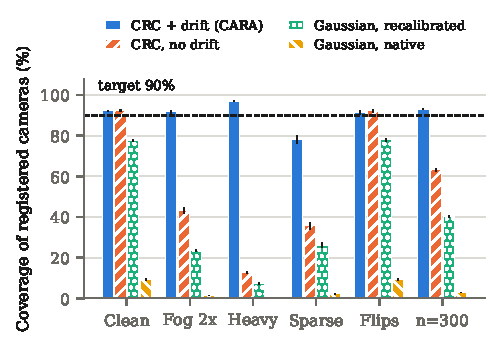
\includegraphics[width=\linewidth]{figs/synth_coverage.pdf}
\caption{Coverage of 90\% per-camera bounds on synthetic scenes (mean and 95\% seed-clustered interval). Gaussian bounds from native or recalibrated uncertainty fail even on clean scenes; calibrated bounds without drift correction fail under shift.}
\label{fig:coverage}
\end{figure}

\subsection{Per-camera bounds}\label{sec:bounds}
\Cref{tab:bounds} and \cref{fig:coverage} compare five ways to bound each camera's error at a 90\% target. Gaussian bounds computed from the native uncertainty cover 9.1\% of cameras on clean scenes (at most 9.2\% in any condition), which is the overconfidence of the front end propagated through averaging; after power-law recalibration they cover 77.7\%. Both collapse under shift (1.3\% and 23.4\% in the fog condition). Calibrated bounds without drift correction reach the target on clean scenes (92.5\%), as \cref{thm:cam} guarantees, and also on the correlated-flip condition (92.4\%), where the guarantee does not formally apply, but fall to 43.2\% (fog), 12.7\% (heavy) and 63.2\% ($n=300$). With the drift factor, coverage is 91.7\% (fog), 97.0\% (heavy) and 93.1\% ($n=300$), and coverage on the hardest quarter of cameras stays within a few points of the marginal value. The price is width: the median bound grows from $1.5^\circ$ to $2.9^\circ$ (fog) and $6.5^\circ$ (heavy), which reflects the real increase in error. The one miss is the sparse condition (78.0\%): the test graphs are sparser than the calibration graphs, which is a shift in structure that a scalar $\hat\rho$ cannot correct.

\begin{figure}[!htbp]
\centering
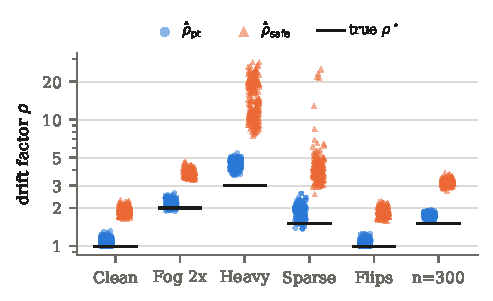
\includegraphics[width=\linewidth]{figs/synth_drift.pdf}
\caption{Label-free drift estimates per test scene (log scale). Bars: true scale factor. $\hat\rho_{\mathrm{safe}}$ is at least the truth in every shifted scene, but loose.}
\label{fig:drift}
\end{figure}

\subsection{Drift estimation}\label{sec:drift}
\Cref{fig:drift} shows both estimators per scene. The point estimate tracks the true factor with a small upward bias in clean and fog scenes (means $1.10$ and $2.17$ for true values $1$ and $2$) and a larger bias in the heavy condition ($4.40$ for $3$), where 35\% outliers contaminate the 20th percentile; the upward bias coincides with over-coverage there (97.0\%). As a detector of shift, $\hat\rho_{\mathrm{pt}}$ separates every shifted condition from clean scenes perfectly (area under the ROC curve (AUROC) $1.00$ for fog, heavy, sparse and $n=300$). It raises no false alarm for correlated flips at unchanged noise (AUROC $0.39$ against clean scenes, i.e.\ slightly \emph{lower} values). The safe estimate was at least the true factor in all 800 shifted scenes; in the fog condition, where the hypotheses of \cref{prop:bracket} hold at population level, this is what the proposition predicts, while in the heavy and sparse conditions it is an empirical observation. It is loose: its mean is $1.91$ on clean scenes and $15.1$ in the heavy condition. Used inside the edge gate, such values admit outliers, and CARA-safe loses accuracy in the heavy condition (AUC@5 $0.155$). We therefore use $\hat\rho_{\mathrm{pt}}$ in the pipeline and reserve $\hat\rho_{\mathrm{safe}}$ for certified alarms.

\begin{table*}[!htbp]
\centering
\caption{1DSfM Notre Dame, 100-camera sub-graphs, calibration and test cameras disjoint; 5 seeds $\times$ 20 test scenes. Same conventions as \cref{tab:synth}; with 5 seeds no comparison can reach the marker threshold.}
\label{tab:real}
\setlength{\tabcolsep}{3.2pt}
\footnotesize
\begin{adjustbox}{max width=\textwidth,max totalheight=0.85\textheight}\begin{tabular}{llcccccc}
\toprule
Condition & Method & AUC@2$^\circ\uparrow$ & AUC@5$^\circ\uparrow$ & Med.\ ($^\circ$)$\downarrow$ & P95 ($^\circ$)$\downarrow$ & Reg.\ (\%)$\uparrow$ & Cat.\ (\%)$\downarrow$\\
\midrule
Clean & L1 & 0.562\,{\scriptsize[0.543,0.590]} & 0.764\,{\scriptsize[0.749,0.782]} & 0.64 & 6.1 & 100.0 & 0.4\\
 & CG & 0.559\,{\scriptsize[0.537,0.589]} & \textbf{0.768\,{\scriptsize[0.752,0.788]}} & 0.67 & 6.1 & 100.0 & 0.6\\
 & CycFilt & 0.559\,{\scriptsize[0.537,0.590]} & 0.768\,{\scriptsize[0.753,0.787]} & 0.66 & 6.1 & 99.9 & 0.7\\
 & GLOMAP-RA & 0.557\,{\scriptsize[0.534,0.588]} & 0.765\,{\scriptsize[0.749,0.785]} & 0.66 & 5.7 & 99.5 & 0.8\\
 & Shonan-H & 0.515\,{\scriptsize[0.495,0.539]} & 0.742\,{\scriptsize[0.727,0.761]} & 0.78 & 7.6 & 100.0 & 0.6\\
 & CG-$\hat\rho$ & 0.555\,{\scriptsize[0.532,0.583]} & 0.767\,{\scriptsize[0.751,0.786]} & 0.68 & 6.1 & 100.0 & 0.6\\
 & CARA-static & 0.550\,{\scriptsize[0.526,0.580]} & 0.742\,{\scriptsize[0.718,0.766]} & 0.60 & 3.9 & 92.1 & 8.1\\
 & CARA & 0.547\,{\scriptsize[0.522,0.576]} & 0.743\,{\scriptsize[0.720,0.765]} & 0.62 & 3.9 & 92.4 & 7.7\\
 & CARA-safe & 0.516\,{\scriptsize[0.493,0.544]} & 0.732\,{\scriptsize[0.710,0.753]} & 0.71 & 4.0 & 93.4 & 6.7\\
\midrule
Noise $\kappa{=}1.5$ & L1 & 0.422\,{\scriptsize[0.401,0.448]} & 0.682\,{\scriptsize[0.661,0.703]} & 1.04 & 6.9 & 100.0 & 0.3\\
 & CG & 0.439\,{\scriptsize[0.418,0.463]} & 0.693\,{\scriptsize[0.671,0.716]} & 0.98 & 7.2 & 100.0 & 0.5\\
 & CycFilt & 0.439\,{\scriptsize[0.418,0.463]} & 0.693\,{\scriptsize[0.671,0.715]} & 0.98 & 7.2 & 99.9 & 0.6\\
 & GLOMAP-RA & 0.440\,{\scriptsize[0.419,0.463]} & \textbf{0.694\,{\scriptsize[0.672,0.715]}} & 0.98 & 6.3 & 99.4 & 1.0\\
 & Shonan-H & 0.428\,{\scriptsize[0.410,0.450]} & 0.687\,{\scriptsize[0.667,0.708]} & 1.02 & 6.6 & 100.0 & 0.3\\
 & CG-$\hat\rho$ & 0.415\,{\scriptsize[0.395,0.435]} & 0.678\,{\scriptsize[0.657,0.699]} & 1.06 & 6.9 & 100.0 & 0.4\\
 & CARA-static & 0.435\,{\scriptsize[0.414,0.460]} & 0.670\,{\scriptsize[0.642,0.697]} & 0.87 & 5.1 & 89.6 & 10.7\\
 & CARA & 0.414\,{\scriptsize[0.393,0.435]} & 0.670\,{\scriptsize[0.646,0.693]} & 1.00 & 5.5 & 95.2 & 4.8\\
 & CARA-safe & 0.398\,{\scriptsize[0.378,0.420]} & 0.658\,{\scriptsize[0.634,0.682]} & 1.06 & 5.5 & 95.2 & 4.8\\
\midrule
Noise $\kappa{=}3$ & L1 & 0.297\,{\scriptsize[0.281,0.312]} & 0.590\,{\scriptsize[0.568,0.613]} & 1.50 & 8.0 & 100.0 & 0.3\\
 & CG & 0.258\,{\scriptsize[0.243,0.274]} & 0.557\,{\scriptsize[0.534,0.579]} & 1.68 & 9.0 & 100.0 & 0.3\\
 & CycFilt & 0.258\,{\scriptsize[0.243,0.274]} & 0.557\,{\scriptsize[0.535,0.581]} & 1.68 & 9.0 & 100.0 & 0.4\\
 & GLOMAP-RA & 0.261\,{\scriptsize[0.246,0.276]} & 0.561\,{\scriptsize[0.539,0.584]} & 1.66 & 8.6 & 99.6 & 0.6\\
 & Shonan-H & 0.302\,{\scriptsize[0.287,0.318]} & \textbf{0.596\,{\scriptsize[0.573,0.619]}} & 1.48 & 8.0 & 100.0 & 0.3\\
 & CG-$\hat\rho$ & 0.298\,{\scriptsize[0.282,0.314]} & 0.591\,{\scriptsize[0.566,0.615]} & 1.51 & 8.0 & 100.0 & 0.3\\
 & CARA-static & 0.152\,{\scriptsize[0.120,0.181]} & 0.318\,{\scriptsize[0.250,0.380]} & 2.24 & 4.7 & 49.0 & 51.0\\
 & CARA & 0.298\,{\scriptsize[0.282,0.314]} & 0.587\,{\scriptsize[0.562,0.613]} & 1.45 & 6.8 & 96.0 & 4.1\\
 & CARA-safe & 0.289\,{\scriptsize[0.272,0.306]} & 0.580\,{\scriptsize[0.554,0.605]} & 1.48 & 6.9 & 95.8 & 4.2\\
\midrule
+15\% outl. & L1 & 0.536\,{\scriptsize[0.515,0.560]} & 0.739\,{\scriptsize[0.721,0.757]} & 0.70 & 15.1 & 100.0 & 2.4\\
 & CG & 0.546\,{\scriptsize[0.524,0.571]} & \textbf{0.753\,{\scriptsize[0.733,0.773]}} & 0.69 & 13.8 & 100.0 & 2.3\\
 & CycFilt & 0.538\,{\scriptsize[0.516,0.564]} & 0.742\,{\scriptsize[0.721,0.762]} & 0.68 & 8.3 & 97.5 & 4.0\\
 & GLOMAP-RA & 0.544\,{\scriptsize[0.522,0.569]} & 0.750\,{\scriptsize[0.731,0.769]} & 0.68 & 12.1 & 99.0 & 3.0\\
 & Shonan-H & 0.492\,{\scriptsize[0.473,0.515]} & 0.724\,{\scriptsize[0.706,0.742]} & 0.84 & 16.3 & 100.0 & 2.3\\
 & CG-$\hat\rho$ & 0.528\,{\scriptsize[0.505,0.554]} & 0.747\,{\scriptsize[0.726,0.768]} & 0.74 & 13.4 & 100.0 & 2.3\\
 & CARA-static & 0.537\,{\scriptsize[0.514,0.562]} & 0.726\,{\scriptsize[0.702,0.750]} & 0.61 & 6.7 & 90.0 & 10.3\\
 & CARA & 0.522\,{\scriptsize[0.499,0.549]} & 0.725\,{\scriptsize[0.706,0.748]} & 0.67 & 8.5 & 91.7 & 8.8\\
 & CARA-safe & 0.474\,{\scriptsize[0.450,0.498]} & 0.700\,{\scriptsize[0.677,0.725]} & 0.81 & 7.5 & 92.8 & 7.6\\
\midrule
$\kappa{=}1.5$+15\% & L1 & 0.387\,{\scriptsize[0.363,0.410]} & 0.650\,{\scriptsize[0.626,0.673]} & 1.17 & 14.3 & 100.0 & 2.7\\
 & CG & 0.424\,{\scriptsize[0.400,0.453]} & 0.675\,{\scriptsize[0.653,0.697]} & 1.03 & 14.3 & 100.0 & 2.5\\
 & CycFilt & 0.420\,{\scriptsize[0.396,0.444]} & 0.666\,{\scriptsize[0.641,0.690]} & 1.01 & 11.0 & 97.5 & 4.3\\
 & GLOMAP-RA & 0.424\,{\scriptsize[0.400,0.450]} & \textbf{0.675\,{\scriptsize[0.652,0.698]}} & 1.02 & 17.3 & 99.4 & 3.1\\
 & Shonan-H & 0.407\,{\scriptsize[0.382,0.436]} & 0.666\,{\scriptsize[0.645,0.689]} & 1.10 & 16.6 & 100.0 & 2.3\\
 & CG-$\hat\rho$ & 0.390\,{\scriptsize[0.365,0.416]} & 0.655\,{\scriptsize[0.634,0.676]} & 1.17 & 13.1 & 100.0 & 2.3\\
 & CARA-static & 0.419\,{\scriptsize[0.394,0.447]} & 0.647\,{\scriptsize[0.618,0.676]} & 0.87 & 5.3 & 85.5 & 14.8\\
 & CARA & 0.389\,{\scriptsize[0.365,0.418]} & 0.646\,{\scriptsize[0.621,0.671]} & 1.07 & 6.6 & 93.3 & 7.0\\
 & CARA-safe & 0.368\,{\scriptsize[0.343,0.396]} & 0.629\,{\scriptsize[0.605,0.656]} & 1.15 & 7.2 & 93.6 & 6.7\\
\bottomrule
\end{tabular}\end{adjustbox}
\end{table*}


\subsection{Real data: 1DSfM Notre Dame}\label{sec:real}
Test sub-graphs have on average 94 cameras and 1,270 edges, of which 17\% disagree with the reference by more than $5^\circ$. \Cref{tab:real} gives a different picture from the synthetic study, and we report it as it is. With the pre-specified configuration, CARA has \emph{lower} AUC@5 than CG in four of five conditions (for example $0.743$ vs.\ $0.768$ on unshifted scenes), in each case in all five seeds; it is higher only under the strongest noise shift ($0.587$ vs.\ $0.557$, all five seeds), where it is still below Shonan-H ($0.596$), CG-$\hat\rho$ ($0.591$) and $L_1$ ($0.590$). GLOMAP-RA ties CG in every condition (within $0.004$), and Shonan-H is within $0.03$ of CG except at $\kappa=3$, where it is the best method. With five seeds, no real-data difference can reach $p<0.05$ in our seed-level test. The AUC deficit comes mostly from abstention: CARA leaves 4--8\% of cameras unregistered, and they count as failures. The abstentions are selective (over all seeds, CG estimates only 21--54\% of the abstained cameras to within $5^\circ$, while its catastrophic rate over all cameras is below 2.5\%), and on the cameras it does register the comparison is mixed. Compared on exactly those cameras, CARA's median error is higher than CG's in four conditions ($0.62^\circ$ vs.\ $0.61^\circ$, $1.00^\circ$ vs.\ $0.92^\circ$, $0.67^\circ$ vs.\ $0.63^\circ$, $1.07^\circ$ vs.\ $0.95^\circ$) and lower at $\kappa=3$ ($1.45^\circ$ vs.\ $1.62^\circ$), and the 95th-percentile errors are $3.9^\circ$ vs.\ $3.4^\circ$ (clean), $5.5^\circ$ vs.\ $5.5^\circ$ ($\kappa=1.5$), $6.8^\circ$ vs.\ $8.0^\circ$ ($\kappa=3$), $8.5^\circ$ vs.\ $3.7^\circ$ (+15\% outliers) and $6.6^\circ$ vs.\ $6.8^\circ$ (both), CARA first.

A diagnostic on 12 additional scenes drawn from seed 0's test half showed that 2-core pruning with $\beta=3$ abstains on many cameras the baseline gets right, and that a less conservative operating point (no core pruning, $\beta=5$), called CARA-lite below, registers 98.5\% of cameras. Because this setting was found on seed 0, we evaluate it only on seeds 1--4 (whose random camera halves overlap seed 0's cameras) and label it post hoc. AUC@5 of CARA-lite vs.\ CG is 0.760 vs.\ 0.769 (clean; higher in 0 of 4 seeds); 0.676 vs.\ 0.692 ($\kappa{=}1.5$; higher in 0 of 4 seeds); 0.592 vs.\ 0.559 ($\kappa{=}3$; higher in 4 of 4 seeds); 0.738 vs.\ 0.753 (+15\% outliers; higher in 0 of 4 seeds); 0.656 vs.\ 0.676 (both; higher in 0 of 4 seeds). It registers 96.8--99.9\% of cameras and its 90\% bounds cover 90.6--99.4\% of registered cameras across the five conditions (80 test scenes per condition).
 Even at this operating point, CARA is less accurate than CG on real sub-graphs except under the strongest noise shift. Two properties of the data explain this. The 1DSfM relative rotations carry no front-end uncertainty, so recalibration and weighting have nothing to use, and the errors are dominated by moderate noise rather than gross outliers, which a well-tuned Geman--McClure kernel already handles. On this dataset CARA's contribution is the calibrated bounds and the drift signal, not accuracy.

\begin{table}[!htbp]
\centering
\caption{Per-camera 90\% bounds on Notre Dame sub-graphs.}
\label{tab:realbounds}
\setlength{\tabcolsep}{2.5pt}
\footnotesize
\resizebox{\columnwidth}{!}{%
\begin{tabular}{llccc}
\toprule
Cond. & Bound & Coverage (\%) & Hard-25\% cov.\ (\%) & Width ($^\circ$)\\
\midrule
Clean & CRC, no drift & 89.0\,{\scriptsize[86.9,91.3]} & 84.2 & 1.35\\
 & CRC + $\hat\rho_{\mathrm{pt}}$ & 89.6\,{\scriptsize[88.2,91.3]} & 85.5 & 1.40\\
 & CRC + $\hat\rho_{\mathrm{safe}}$ & 90.4\,{\scriptsize[88.9,92.0]} & 85.6 & 1.57\\
\midrule
Noise $\kappa{=}1.5$ & CRC, no drift & 87.0\,{\scriptsize[84.8,89.6]} & 80.3 & 1.58\\
 & CRC + $\hat\rho_{\mathrm{pt}}$ & 97.6\,{\scriptsize[96.1,98.7]} & 95.9 & 3.88\\
 & CRC + $\hat\rho_{\mathrm{safe}}$ & 96.8\,{\scriptsize[95.4,97.9]} & 94.6 & 3.30\\
\midrule
Noise $\kappa{=}3$ & CRC, no drift & 81.0\,{\scriptsize[76.5,85.7]} & 77.5 & 2.84\\
 & CRC + $\hat\rho_{\mathrm{pt}}$ & 99.3\,{\scriptsize[99.1,99.5]} & 99.2 & 6.60\\
 & CRC + $\hat\rho_{\mathrm{safe}}$ & 98.7\,{\scriptsize[98.3,99.2]} & 98.0 & 5.45\\
\midrule
+15\% outl. & CRC, no drift & 90.2\,{\scriptsize[88.3,92.2]} & 84.5 & 1.47\\
 & CRC + $\hat\rho_{\mathrm{pt}}$ & 94.0\,{\scriptsize[92.4,95.6]} & 90.0 & 1.88\\
 & CRC + $\hat\rho_{\mathrm{safe}}$ & 95.2\,{\scriptsize[93.9,96.5]} & 91.5 & 2.37\\
\midrule
$\kappa{=}1.5$+15\% & CRC, no drift & 89.6\,{\scriptsize[88.2,91.7]} & 83.9 & 1.64\\
 & CRC + $\hat\rho_{\mathrm{pt}}$ & 98.4\,{\scriptsize[97.8,99.0]} & 97.3 & 4.86\\
 & CRC + $\hat\rho_{\mathrm{safe}}$ & 97.8\,{\scriptsize[97.3,98.2]} & 95.7 & 4.32\\
\bottomrule
\end{tabular}}
\end{table}


\paragraph*{Bounds on real data} The guarantees of \cref{sec:theory} do not formally apply here (calibration and test cameras come from different halves, and sub-graphs overlap), so coverage is an empirical question. \Cref{tab:realbounds} shows that calibrated bounds hold close to the target on unshifted real scenes (89.6\% for a 90\% target), with lower coverage on the hardest quarter of cameras (85.5\%), which is the conditional failure that marginal guarantees permit~\cite{pathak2026adaptive}. Under noise shift, bounds without drift correction fall to 87.0\% ($\kappa=1.5$) and 81.0\% ($\kappa=3$). With $\hat\rho_{\mathrm{pt}}$ they over-cover (97.6\% and 99.3\%), because the drift factor overestimates the nominal shift ($3.38$ vs.\ $1.80$ and $5.97$ vs.\ $3.16$). Here the shift adds noise to heterogeneous, heavy-tailed intrinsic errors; the most accurate edges, which set the low quantile in \eqref{eq:rho}, are inflated proportionally more, so \cref{ass:scale} is violated and $\hat\rho$ overshoots. In these runs the overshoot produced wider bounds, not missed coverage. Injected outliers alone also raise $\hat\rho_{\mathrm{pt}}$ (mean $1.47$ at unchanged noise), because the total outlier fraction reaches 30\%.

\paragraph*{Full graph} On the complete 715-camera graph, using the seed-0 calibration from 100-camera sub-graphs (whose cameras are part of this graph), CARA, CG and GLOMAP-RA reach the same AUC@5 ($0.843$, $0.842$ and $0.842$; Shonan-H $0.821$); $L_1$ has the best AUC@2 ($0.666$ vs.\ $0.658$ for CARA) and the lowest median error ($0.49^\circ$ vs.\ $0.51^\circ$). CARA has lower mean and 95th-percentile error over its registered cameras ($0.95^\circ$ vs.\ $1.12^\circ$ and $2.08^\circ$ vs.\ $2.32^\circ$ for CG over all cameras), but it abstains on 1.1\% of cameras and its catastrophic rate is higher (1.4\% vs.\ 0.4\%). It keeps 91.5\% of inlier edges and rejects 96.6\% of edges that disagree with the reference by more than $5^\circ$, and it takes 70\,s against 11\,s for CG in our single-threaded Python implementation (runtime scaling in \supp{4}) and 3.7\,s for the compiled GLOMAP-RA.

\subsection{Real images with a learned front end: ETH3D and VGGT}\label{sec:eth3d}
These experiments remove the two main gaps of the previous ones: the relative rotations and their uncertainty come from a learned network run on real images, and the degradations act on pixels, not on rotations.

\paragraph{Common protocol} We use the 13 scenes of the ETH3D high-resolution multi-view training set~\cite{schops2017eth3d}. A sub-scene is a random set of 12 images, and its view graph links each image to its 6 nearest cameras by viewing direction and position (about 40 edges). VGGT-1B~\cite{wang2025vggt} is run on every image pair (inputs downscaled to at most 1024\,px, then to VGGT's 518\,px), and the relative rotation is read from its camera head. The edge uncertainty is pre-registered as $\hat\sigma_{ij}=1/\mathrm{median}$ of VGGT's depth confidence over both images. Test conditions are: clean; fog rendered with the atmospheric scattering model at median transmission $t\in\{0.7,0.5,0.3\}$, using depth predicted by VGGT on the clean image; low light (Poisson--Gaussian noise at $0.3$ and $0.15$ of the linear exposure); and synthetic rain streaks. Calibration uses 140 clean sub-scenes (split $20/40/40/40$ into $\mathcal{D}_{\mathrm{fit}},\mathcal{D}_{\mathrm{edge}},\mathcal{D}_{\mathrm{res}},\mathcal{D}_{\mathrm{cam}}$ and reshuffled for each of 5 seeds), and calibration and test sub-scenes never come from the same place. Sub-scenes with a disconnected view graph are reduced to their largest component for every method. Edges with error above $5^\circ$ count as outliers. Methods, configuration and metrics are those of \cref{sec:protocol}; ConfW uses VGGT's confidence. Seeds only reshuffle the calibration splits, so the unit of inference is the test scene: we average over seeds and sub-scenes per scene and use an exact sign-flip test over scenes.

\paragraph{First run} A first run with a fixed split (6 calibration and 7 test scenes, 490 test graphs) is reported in \supp{1}. CARA's mean AUC@5$^\circ$ was above CG, GLOMAP-RA and Shonan-H in every condition, but not significantly over 7 scenes, and ConfW was as accurate. The bounds covered 88.6\% of registered cameras on clean held-out scenes, but 78.9--85.2\% under degradation and 68--74\% on the quarter of cameras with the largest $u_i$. The run also showed that VGGT is robust to these degradations: they mainly add gross failures instead of rescaling inlier noise, which \cref{ass:scale} does not describe, and the pre-registered median confidence sits on VGGT's confidence floor for 55\% of edges. These findings motivated the extensions of \cref{sec:ext}.


\subsection{Confirmatory run: 13 scenes and the extensions}\label{sec:v2}
The first ETH3D run exposed two weaknesses: bounds that under-cover under degradation, most of all on hard cameras, and too few test scenes for significance. We designed E1 and E2 (\cref{sec:ext}) on the calibration scenes of that run, with injected failures and leave-one-scene-out validation, and then evaluated them on its test scenes, which had been seen in aggregate before. To test them without that bias, we computed a second, independent set of VGGT outputs and fixed six hypotheses, the primary variant and all settings before those outputs existed (the pre-registration file is reproduced in \supp{7} and released with the code). The development of E1 and E2 and their results on the first run are in \supp{5}, and their behaviour on synthetic scenes in \supp{6}.

\paragraph*{Protocol (E4)} All 13 ETH3D scenes are test scenes in turn: for each, CARA is calibrated on 140 clean sub-scenes of the other 12 scenes (leave-one-scene-out) and tested on 8 new random sub-scenes of 12 cameras (seed 3, none shared with the first run) under the same 7 conditions, 728 test graphs in total (21 of them keep 7 or 11 cameras after restriction to the largest component). Seven of the 13 places are the first run's test scenes, with different images selected. Each file also stores VGGT's relative translation, the relative rotation of the previous camera-head iteration, and per-image confidence statistics. Everything else follows \cref{sec:eth3d}; the unit of inference is the test scene (13 scenes, smallest two-sided $p=2^{-12}$). The clean edges have a median inlier error of $0.74^\circ$, 21.1\% exceed $5^\circ$ and 11.7\% exceed $30^\circ$; under low light at $0.15$ the latter reaches 19.4\%.

\paragraph*{E3: learned edge uncertainty} From the stored signals we form five edge features (median confidence over both images, the worst and the best image's mean log confidence, the worst image's 10\% confidence quantile, and the log angle between the last two camera-head iterations) and fit $\log\hat\sigma$ as a linear function of them to the log error of inlier edges on $\mathcal{D}_{\mathrm{fit}}$ only. For numerical safety the prediction is clipped to $[10^{-4},\pi]$\,rad. This guard was added after the run-2 outputs had been computed and the first evaluation attempt failed on a fold that produced a zero uncertainty; it changes no other setting, but it is a deviation from the pre-registration. Separating outlier edges ($>5^\circ$), the learned $\hat\sigma$ reaches an AUROC of $0.873$ against $0.701$ for the pre-registered median (13 of 13 scenes). The worst-image mean log confidence alone reaches $0.853$ and, unexpectedly, the small change between camera-head iterations (median $0.028^\circ$, quantized by the half-precision arithmetic of the T4 GPU) reaches $0.824$; the 10\% quantile sits on VGGT's confidence floor and carries no information ($0.505$).

\input{tables/v2_acc}

\paragraph*{Accuracy with 13 scenes} \Cref{tab:v2acc} reports AUC@5$^\circ$. With the pre-registered $\hat\sigma$, CARA's mean is above CG in all seven conditions (by $0.012$ to $0.032$) and above GLOMAP-RA and Shonan-H in all seven. Over the 13 scenes, pooled across conditions, CARA beats CG on 9 scenes ($+0.026$, $p=0.051$), GLOMAP-RA on 10 ($p=0.028$), Shonan-H on 10 ($p=0.002$) and CG-$\hat\rho$ on 9 ($p=0.037$). These comparisons were not among the pre-registered hypotheses and are not corrected for multiplicity. ConfW remains as accurate as CARA ($-0.002$, $p=0.84$). With the learned $\hat\sigma$ (E3), CARA gains $0.020$ (11 of 13 scenes, $p=0.018$; not in fog $0.3$) and ConfW gains $0.029$; the most accurate method in five of seven conditions is ConfW with the learned uncertainty, and CARA with it is not significantly different ($-0.010$, $p=0.33$). Better uncertainty helps both uncertainty-aware methods we tested; CARA's gates do not add accuracy on top of good weights.

\input{tables/v2_bounds}

\paragraph*{Per-camera bounds} \Cref{tab:v2bounds} pools the six degraded conditions, and \cref{fig:v2}(a) shows each condition. The unmodified bounds cover 87.9\% of registered cameras and 81.8\% of the hardest quarter; with leave-one-scene-out calibration over 12 varied scenes they are wide (median $15.6^\circ$ when not flagged) and flag 36\% of cameras. E2 raises coverage on the hardest quarter to 92.8\% ($+11.0$ points, 11 of 13 scenes) and overall coverage to 90.9\% ($+3.1$, 7 of 13 scenes), halves the unflagged width to $8.1^\circ$, and flags 78\% of the cameras whose error exceeds $30^\circ$, against 45\% without it. The cost is a higher flag rate (42\% against 36\%): only about one flagged camera in five is actually wrong by more than $30^\circ$, so on these small graphs a 90\% guarantee is bought by declaring many correct cameras unreliable. E1 alone adds 1.5 points of coverage (12 of 13 scenes) at the price of wider bounds. Combining E1 with E2 gives narrower bounds and fewer flags (31\%) but covers less than E2 alone, and less than the unmodified bounds overall (86.7\%). E1+E2a denotes E1 with the learned normalizer but without groups. The secondary variant E2u, which groups cameras by $u_i$ without the learned normalizer, covers more than E2 (92.5\% overall and on hard cameras; hard coverage above the unmodified bounds on all 13 scenes) but flags 61\% of cameras. As in the first run, the learned normalizer does not rank catastrophic cameras better than $u_i$ (AUROC $+0.002$); its benefit is a better split into groups.

\begin{figure}[!htbp]\centering
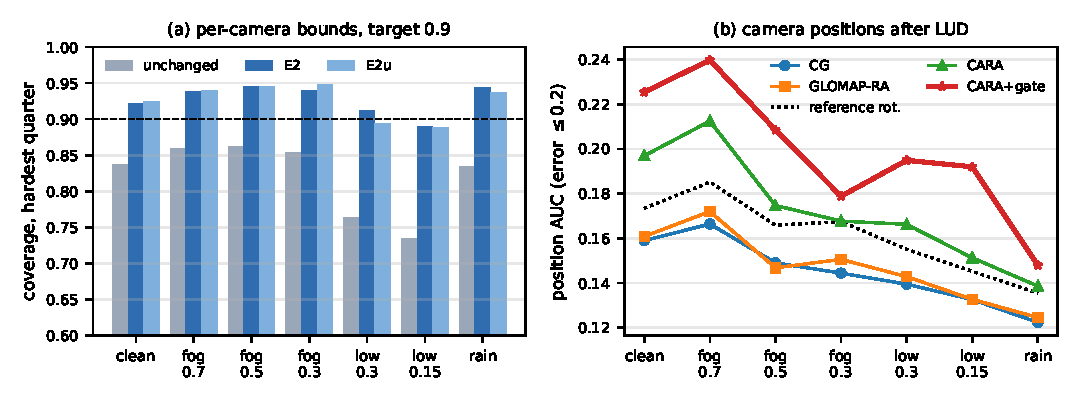
\includegraphics[width=\linewidth]{figs/v2.pdf}
\caption{Confirmatory ETH3D run (13 scenes). (a) Coverage of the per-camera bounds on the quarter of cameras with the largest $u_i$, for the unchanged bounds and the difficulty-conditional variants E2 and E2u; dashed line: target. (b) Position AUC after translation averaging by least unsquared deviations (LUD) with each method's rotations; CARA+gate uses only CARA's accepted edges, and the dotted line uses the reference rotations with all edges.}\label{fig:v2}
\end{figure}

\input{tables/v2_trans}

\paragraph*{E5: effect on camera positions} We rotate VGGT's relative translations by each method's global rotations and solve translation averaging by least unsquared deviations (LUD)~\cite{ozyesil2015robust} on the same graph, then align to the reference centres by a similarity and divide the error by the median distance of the cameras to their centroid. \Cref{tab:v2trans} and \cref{fig:v2}(b) show that all methods give large position errors on these 12-camera graphs (median $0.32$ to $0.44$ of the scene radius), because many VGGT translation directions are wrong. CARA's rotations alone raise the position AUC over CG on all 13 scenes ($+0.028$, $p=0.0002$), partly because edges of unregistered cameras are dropped, and restricting LUD to CARA's accepted edges adds another $0.026$ (9 of 13 scenes, $p=0.073$). Together the gain over CG is $+0.053$ (12 of 13 scenes, $p=0.0005$), and the AUC exceeds that obtained with the reference rotations on all edges ($0.225$ against $0.173$ on clean scenes), so removing edges matters as much as correcting rotations. These AUC comparisons were not pre-registered. On the median position error, CARA with its gate is better than CG on 9 of 13 scenes ($p=0.030$), but not better than the reference rotations.

\input{tables/v2_hyp}

\paragraph*{Pre-registered hypotheses} \Cref{tab:v2hyp} lists the six hypotheses. The pre-registration fixed one-sided tests for H1--H3 but did not state the sidedness for H4--H6, which are directional; we report the conservative two-sided values. With one-sided values, H4 and H6 would also survive Holm correction ($0.036$ and $0.045$). The guarantee of \cref{cor:group} concerns the three groups by $v_i$; H1 measures the top quarter by $u_i$, a related but different set. After Holm correction two hypotheses hold: E2 raises coverage of the hardest cameras (H1) and the learned uncertainty separates outlier edges better (H5). Three are supported at the unadjusted level but not after correction: overall coverage under E2 (H2), accuracy with the learned uncertainty (H4) and the position error with CARA's edge set (H6). H3, a better ranking of catastrophic cameras by the learned normalizer, fails.


\subsection{Label-free audit of uncertainty}\label{sec:audit}
The drift statistic can also audit uncertainties that come with a dataset. If per-axis standard deviations were correct, the normalized cycle angle of a clean triangle would follow a Maxwell ($\chi_3$) law to first order, so $\hat\kappa(p)=\operatorname{Q}_p(t)/\operatorname{Q}_p(\chi_3)$ estimates their scale error without reference poses. On synthetic scenes with known factors $1, 2.4, 5, 10$ and no outliers, $\hat\kappa(0.05)$ returns $1.00, 2.43, 4.95, 9.97$. With 20\% outlier edges it overestimates by $28\%$, which is the value \cref{prop:bracket} predicts: 49\% of triangles are then contaminated and $\operatorname{Q}_{0.05/0.51}(\chi_3)/\operatorname{Q}_{0.05}(\chi_3)=1.28$. We attempted to apply the audit to the rotation covariances released with~\cite{zhang2023revisiting} for Madrid Metropolis, but the relative rotations stored in that file disagree with the 1DSfM relative rotations for the same pairs by a median of about $29^\circ$ and do not close around cycles under either orientation convention, so we could not establish the frame in which the covariances are expressed. We therefore report no result for real covariances.

\begin{figure}[!htbp]
\centering
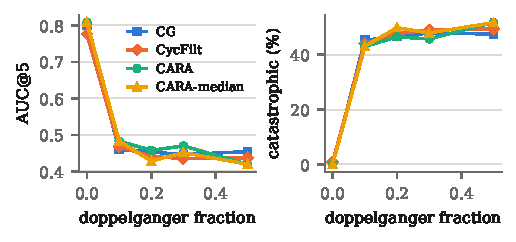
\includegraphics[width=\linewidth]{figs/dop.pdf}
\caption{Structured doppelgangers on a ring of 100 cameras around a symmetric object (5 seeds $\times$ 10 scenes per point). Spurious look-alike edges map a camera to its mirror twin and are mutually cycle-consistent. All methods fail once they are present.}
\label{fig:dop}
\end{figure}

\subsection{Structured doppelgangers}\label{sec:dop}
We place 100 cameras on a circle around an object with a $180^\circ$ symmetry and add spurious edges between cameras in the front half and cameras in the back half whose mirror twin would overlap them, with the relative rotation of the twin. These edges agree with each other around every cycle they share, so no cycle test can reject them. Without them, CARA reaches AUC@5 $0.808$ against $0.799$ for CG. With 10\% of the candidate look-alike pairs added (65 of 781 edges), every method fails: 43--45\% of cameras become catastrophic, CARA rejects only 12\% of the spurious edges, and bound coverage falls to 56\%. The picture does not change at higher fractions (\cref{fig:dop}). Neither the median triangle score nor the drift factor helps. This is the limit stated in \cref{rem:guar}: calibrated cycle tests do not replace doppelganger classifiers~\cite{cai2023doppelgangers,xiangli2025doppelgangerspp}, and the bounds are not valid when the error mechanism produces consistent wrong evidence.




\section{Discussion and Limitations}\label{sec:discussion}

\paragraph*{What the guarantees buy} \Cref{thm:edge,thm:res,thm:cam} hold for any front end and any uncertainty proxy when calibration and test scenes are exchangeable, because every threshold is calibrated on held-out scenes. In practice, Gaussian bounds from native or recalibrated uncertainty cover far less than their nominal level, while calibrated bounds reach it on clean scenes, and the label-free drift factor keeps them near it under a scale shift. Consensus bridging turns a silent wrong pose into an explicit abstention.

\paragraph*{When a tuned robust baseline is preferable} Three conditions limit the claims. (i) On sparse graphs, CARA's gates and $2$-core pruning remove support that the robust baseline still uses, which raises abstentions and catastrophic errors; CG with our drift-scaled kernel alone is better there. When the average degree is low, a practitioner should reduce the core order or disable pruning; this choice can be calibrated like the other thresholds. (ii) When the graph structure shifts rather than the noise level (the sparse condition is calibrated on denser graphs), per-camera coverage falls below target, because \cref{ass:scale} does not describe that shift and no scalar $\hat\rho$ can correct it. Calibrating on scenes whose graph statistics match the deployment, or weighting calibration scenes by graph similarity~\cite{tibshirani2019covariate}, are the natural fixes. (iii) Mutually consistent wrong edges pass the cycle test by construction, and the low triangle quantile, chosen to protect inliers from contamination, makes this worse; a median resists it but loses inliers. Learned doppelganger classifiers~\cite{cai2023doppelgangers,xiangli2025doppelgangerspp} or geometric reliability features~\cite{ahmedt2026geocond} address this failure mode and can enter the score as additional inputs.

\paragraph*{Drift estimation and misspecification} $\hat\rho_{\mathrm{safe}}$ was at least the true factor in every shifted synthetic scene, as \cref{prop:bracket} predicts where its hypotheses hold, but it is loose, and under heavy contamination its large values open the edge gate to outliers. We therefore recommend $\hat\rho_{\mathrm{pt}}$ for estimation and $\hat\rho_{\mathrm{safe}}$ as a certified alarm or for bounds only. On Notre Dame the added noise is not a pure rescaling of heterogeneous intrinsic noise, and $\hat\rho_{\mathrm{pt}}$ overestimates the nominal factor; in our runs this produced over-coverage rather than under-coverage, but \cref{cor:mono} does not guarantee that direction for the full pipeline.

\paragraph*{Limits of the evaluation} The synthetic generator follows the model CARA is built on (isotropic Lie-algebra noise, overconfident but rank-correlated uncertainty, a scale shift), and its overconfidence factor comes from an audit of per-pixel pointmap confidences rather than relative-rotation uncertainty. On Notre Dame there is no front-end uncertainty and CARA is not more accurate than the robust baseline. The guarantees do not formally apply there either: calibration and test scenes come from disjoint camera halves and overlapping sub-graphs, so they are neither exchangeable nor independent, and the full-graph run includes the calibration cameras.

On ETH3D with VGGT, the only experiment with learned uncertainty on real images, the graphs are small (12 cameras), there are 13 scenes, and the degradations are rendered, with fog using depth predicted by VGGT itself. CARA's accuracy gain over CG is marginal ($p=0.051$, uncorrected) and absent against ConfW. Without the extensions, its bounds under-cover under degradation (87.9\% overall, 81.8\% on the hardest quarter; 78.9--85.2\% overall in the first run, \supp{1}) because the shift raises the rate of gross failures, which \cref{ass:scale} does not model. \Cref{sec:ext,sec:v2} trace this to camera-level failures that cancel in every cycle and close the gap on hard cameras with difficulty-conditional bounds; the price is a high flag rate (42\% of cameras, about four in five of them correct), and the learned normalizer does not detect wrong cameras better than $u_i$. The confirmatory run shares seven places with the first run, and E3's clipping guard was added after its outputs had been computed. Its leave-one-scene-out design is not exchangeable either: calibration sub-scenes come from 12 clean places, while each test place is unseen and degraded.

Besides our own implementations, we compare with two released ones (GLOMAP-RA and Shonan-H); released implementations of uncertainty-aware and hierarchical averaging~\cite{zhang2023revisiting,lee2022hara} and of the certifiable anisotropic solver~\cite{olsson2025certifiably} are still missing. The robustness grid in \supp{3} shows how accuracy and coverage change when noise and outlier rates move away from the calibration setting.

\paragraph*{Next steps} The most important missing evaluations are larger image collections (IMC PhotoTourism, Tanks and Temples), real rather than rendered adverse conditions such as ACDC~\cite{sakaridis2021acdc}, and a second front end such as MASt3R. Detecting a misread image directly, for example from disagreement between its pairwise and multi-view reconstructions, is the most promising route to informative bounds for hard cameras. The aggregation of per-pixel confidence into an edge-level $\hat\sigma$ also matters: on ETH3D a median of VGGT's depth confidence saturates at its floor on most edges, while a mean log-confidence separates outliers far better, so learning this aggregation on calibration scenes is a natural extension. The same structure (cycle or residual nonconformity, scene-level risk control, a drift factor and consensus-based registration) extends to translation averaging and to GLOMAP-style global positioning~\cite{pan2024glomap}, where residuals are point-to-ray distances. The guarantees are marginal over scenes; conditional guarantees per camera difficulty, as advocated in~\cite{pathak2026adaptive}, remain an open problem for jointly estimated reconstructions.


\section{Conclusion}\label{sec:conclusion}
CARA turns front-end uncertainty in rotation averaging from an input that is either trusted or ignored into a quantity that is recalibrated, tested against cycle closure, rescaled when the data drift, and converted into per-camera bounds with finite-sample guarantees. On synthetic scenes with overconfident, drifting uncertainty, it is more accurate than a strong robust baseline on all but sparse graphs, and its bounds stay close to their target under noise shifts. On 1DSfM Notre Dame, without front-end uncertainty, it gives bounds near their target and a shift signal, though not higher accuracy, and neither it nor any baseline survives structured doppelgangers.

With a learned front end on real images (VGGT on ETH3D), the bounds are close to their target on clean held-out scenes. Under rendered fog, low light and rain they fall short on hard cameras, and we trace this to camera-level failures that cancel in every cycle. Difficulty-conditional bounds raise coverage of the hardest cameras from 81.8\% to 92.8\% in a pre-registered run over 13 scenes, at the cost of flagging many correct cameras. A learned edge uncertainty separates outlier edges much better and raised the accuracy of both uncertainty-aware methods we tested, although not significantly after multiplicity correction; in an analysis that was not pre-registered, CARA's rotations and accepted edges raised the position accuracy after translation averaging. Accuracy gains over robust and confidence-weighted averaging remain small ($p=0.051$ against CG, uncorrected).

The next steps are a signal that detects misread images directly, larger view graphs, a second front end, and bundle adjustment under real adverse conditions.


\section*{CRediT authorship contribution statement}
\textbf{Siva Ramakrishna Jeevakala:} Conceptualization, Methodology, Software, Validation, Formal analysis, Investigation, Data curation, Visualization, Writing -- original draft, Writing -- review \& editing. \textbf{A. P. Siva Kumar:} \textcolor{red}{[ROLES, e.g. Supervision, Validation, Writing -- review \& editing]}.

\section*{Declaration of competing interest}
The authors declare that they have no known competing financial interests or personal relationships that could have appeared to influence the work reported in this paper.

\section*{Funding}
This research did not receive any specific grant from funding agencies in the public, commercial, or not-for-profit sectors.

\section*{Data availability}
The implementation, the calibration and test splits, the pre-registration file, all VGGT outputs used in the ETH3D experiments, the raw per-scene results and the scripts that regenerate every table and figure are available at \textbf{[REPOSITORY URL]} and archived at \textbf{[ZENODO DOI]}. The ETH3D images are available from the ETH3D benchmark~\cite{schops2017eth3d}; the Notre Dame data are from 1DSfM~\cite{wilson2014robust} in the distribution of~\cite{chatterjee2018robust}. The VGGT weights are distributed by their authors under their own licence.

\section*{Declaration of generative AI and AI-assisted technologies in the manuscript preparation process}
During the preparation of this work the authors used Claude (Anthropic) to assist with the literature survey, code development, experimental analysis and manuscript drafting. The authors directed the study, reviewed and verified the methods, results and text, and take full responsibility for the content of the published article.

\section*{Acknowledgements}
The authors thank the creators of the ETH3D benchmark, of the 1DSfM data and of VGGT for making their data and models publicly available. The GPU experiments were run on Google Colab.


\bibliographystyle{elsarticle-num}
\bibliography{refs}

\appendix
\section{Proofs}\label{app:proofs}

\begin{lemma}[Conformal risk control~\cite{angelopoulos2024crc}]\label{lem:crc}
Let $L_1,\dots,L_{N+1}:\mathbb{R}\cup\{+\infty\}\to[0,1]$ be exchangeable random functions that are non-increasing and right-continuous with $L_t(+\infty)=0$, and let $\hat\lambda$ be defined by \eqref{eq:crc} from $L_1,\dots,L_N$. Then $\mathbb{E}[L_{N+1}(\hat\lambda)]\le\alpha$.
\end{lemma}
\begin{proof}
Let $\hat R_{N+1}(\lambda)=\frac{1}{N+1}\sum_{t=1}^{N+1}L_t(\lambda)$ and $\lambda'=\inf\{\lambda:\hat R_{N+1}(\lambda)\le\alpha\}$. Because $L_{N+1}\le1$, $\hat R_{N+1}(\lambda)\le\frac{N}{N+1}\hat R_N(\lambda)+\frac{1}{N+1}$ for every $\lambda$. By right-continuity the infimum in \eqref{eq:crc} is attained, so $\hat R_{N+1}(\hat\lambda)\le\alpha$, which gives $\lambda'\le\hat\lambda$, and by monotonicity $L_{N+1}(\hat\lambda)\le L_{N+1}(\lambda')$. The threshold $\lambda'$ is a symmetric function of $(L_1,\dots,L_{N+1})$, so by exchangeability $\mathbb{E}[L_{N+1}(\lambda')]=\mathbb{E}[\hat R_{N+1}(\lambda')]\le\alpha$, where the last step uses right-continuity again.
\end{proof}

In our losses $L(+\infty)=0$ by construction (scores are finite, and an infinite residual satisfies $r\le+\infty$). A scene with an empty set of inlier edges or registered cameras has $L\equiv0$; this case did not occur in our experiments.

\begin{proof}[Proof of \cref{thm:edge}]
Condition on $\mathcal{D}_{\mathrm{fit}}$; then $g$ and $\hat F_C$ are fixed and the round-one scores (including the scene's own $\hat\rho$) are a fixed measurable function of each scene. The losses \eqref{eq:edgeloss} of the scenes in $\mathcal{D}_{\mathrm{edge}}$ and of the test scene are therefore exchangeable, take values in $[0,1]$, and are non-increasing and right-continuous step functions of $\lambda$. \Cref{lem:crc} gives $\mathbb{E}[L^{\mathrm{edge}}_{Z_{N+1}}(\hat\lambda_{\mathrm{edge}})]\le\alpha_{\mathrm{edge}}$ for round one. Round two only adds edges to the accepted set, so the set of rejected testable inliers after rescue is a subset of the round-one rejected set and its fraction is no larger. Removing the conditioning preserves the bound. In the implementation $\hat R_N$ is a step function whose jumps lie at calibration scores, so minimizing over the finite grid of calibration scores and $0$ returns the infimum in \eqref{eq:crc}.
\end{proof}

\begin{proof}[Proof of \cref{thm:res}]
Condition on $\mathcal{D}_{\mathrm{fit}}\cup\mathcal{D}_{\mathrm{edge}}$. The first solve, including gating with the now fixed $\hat\lambda_{\mathrm{edge}}$, pruning and bridging with the fixed constant $\beta$, is a fixed function of each scene, so the residual losses are exchangeable across $\mathcal{D}_{\mathrm{res}}$ and the test scene, bounded in $[0,1]$, non-increasing and right-continuous; \cref{lem:crc} applies.
\end{proof}

\begin{proof}[Proof of \cref{thm:cam}]
Condition on the first three splits. The full pipeline is then a fixed function of the scene, so the losses \eqref{eq:camloss} of the scenes in $\mathcal{D}_{\mathrm{cam}}$ and of the test scene are exchangeable, lie in $[0,1]$, and are non-increasing and right-continuous in $\lambda$ because $u_i>0$. Apply \cref{lem:crc}.
\end{proof}

\begin{proof}[Proof of \cref{lem:equiv}]
Write $\tilde R_{ij}=R_{ij}\operatorname{Exp}(\rho\eta_{ij})$. For a triangle $(i,j,k)$ of inlier edges, $C_{ijk}=\operatorname{Exp}(\rho\,\mathrm{Ad}_1\eta_{ki})\operatorname{Exp}(\rho\,\mathrm{Ad}_2\eta_{jk})\operatorname{Exp}(\rho\eta_{ij})$ with rotation matrices $\mathrm{Ad}_1,\mathrm{Ad}_2$ that depend only on the true rotations. By the Baker--Campbell--Hausdorff formula, $\operatorname{Log}C_{ijk}=\rho(\eta_{ij}+\mathrm{Ad}_2\eta_{jk}+\mathrm{Ad}_1\eta_{ki})+O(\rho^2\|\eta\|^2)$, so its norm scales by $\rho$ to first order, and so does every quantile of such norms divided by quantities that do not depend on $\rho$; this is (a) for scores whose low quantile is attained on inlier triangles. By hypothesis $\hat\rho$ scales by $\rho$, which gives (b) for scores; for residuals it follows from (c). For (c), linearize one IRLS step around the true rotations: the update solves $\sum_{(i,j)}w_{ij}(\omega_j-\omega_i-d_{ij})=0$ with $d_{ij}$ linear in the noise and weights $w_{ij}=\pi_{ij}\kappa(\|d_{ij}\|/(c\hat\rho))$. The Geman--McClure factor is invariant when $d$ and $\hat\rho$ both scale by $\rho$; the $L_1$ factor $1/\|d\|$ and the prior weights $\pi_{ij}\propto(\hat\rho\sigma_{ij})^{-2}$ scale uniformly and cancel. For an accepted outlier edge the residual $r_{\mathrm{out}}$ does not shrink with the noise, and its Geman--McClure weight is $\pi\,(c\hat\rho/r_{\mathrm{out}})^4(1+O((c\hat\rho/r_{\mathrm{out}})^2))$, which does not scale like the inlier weights; its pull on the solution is therefore not proportional to $\rho$. Hence the fixed point scales by $\rho$ up to a term of order $\max_{\mathrm{out}}(c\hat\rho/r_{\mathrm{out}})^4$ contributed by accepted outliers, which vanishes when no outlier edge enters the solve and is negligible when $r_{\mathrm{out}}\gg c\hat\rho$; the same holds for the camera errors. For (d), $u_i$ scales by $\hat\rho$. When no decision lies on a threshold, a small enough noise level keeps every decision unchanged, and each loss, being a function of decisions and of the ratios above, is unchanged.
\end{proof}

\begin{proof}[Proof of \cref{prop:bracket}]
For every $t$, $G(t)\ge(1-\varepsilon)F_T(t)$ and $G(t)\le(1-\varepsilon)F_T(t)+\varepsilon$. At $t_1=\operatorname{Q}_{p/(1-\varepsilon)}(F_T)$ the first inequality gives $G(t_1)\ge p$, so $\operatorname{Q}_p(G)\le t_1=\rho^\star\operatorname{Q}_{p/(1-\varepsilon)}(F_C)$. For $t<t_2=\operatorname{Q}_{(p-\varepsilon)/(1-\varepsilon)}(F_T)$ we have $F_T(t)<(p-\varepsilon)/(1-\varepsilon)$ and the second inequality gives $G(t)<p$, so $\operatorname{Q}_p(G)\ge t_2=\rho^\star\operatorname{Q}_{(p-\varepsilon)/(1-\varepsilon)}(F_C)$. Rearranging both gives the bracket. The map $\varepsilon\mapsto(p-\varepsilon)/(1-\varepsilon)$ is decreasing for $p<1$, so replacing $\varepsilon$ by $\bar\varepsilon\ge\varepsilon$ lowers the denominator and raises the upper end, which proves $\hat\rho_{\mathrm{safe}}\ge\rho^\star$ at the population level. The outer $\max(1,\cdot)$ only increases it.
\end{proof}

\begin{proof}[Proof of \cref{cor:mono}]
In round one the gate accepts $e$ iff $s_e/\hat\rho\le\hat\lambda_{\mathrm{edge}}$ or $s_e$ is undefined, a condition that is monotone in $\hat\rho$. For a fixed accepted set, $B_i=\hat\lambda_{\mathrm{cam}}\hat\rho\,u_i^{(1)}$ with $u_i^{(1)}$ computed at $\hat\rho=1$.
\end{proof}


\end{document}
